\documentclass[a4paper,12pt]{article}

\usepackage[utf8]{inputenc}
\usepackage[T1]{fontenc}
\usepackage[english]{babel}
\usepackage{times}
\usepackage{graphicx}

\setlength{\parindent}{0pt}
\setlength{\parskip}{2ex}

\title{SBrick Plus adapter types, parts, assembly steps}

\author{VENGIT Ltd.}

\begin{document}

\maketitle

\pagebreak

\section{Relevant LEGO product lines}

This document contains references to various LEGO product lines. In the
following pages there are descriptions and images of these product lines.

\subsection{LEGO Technic}

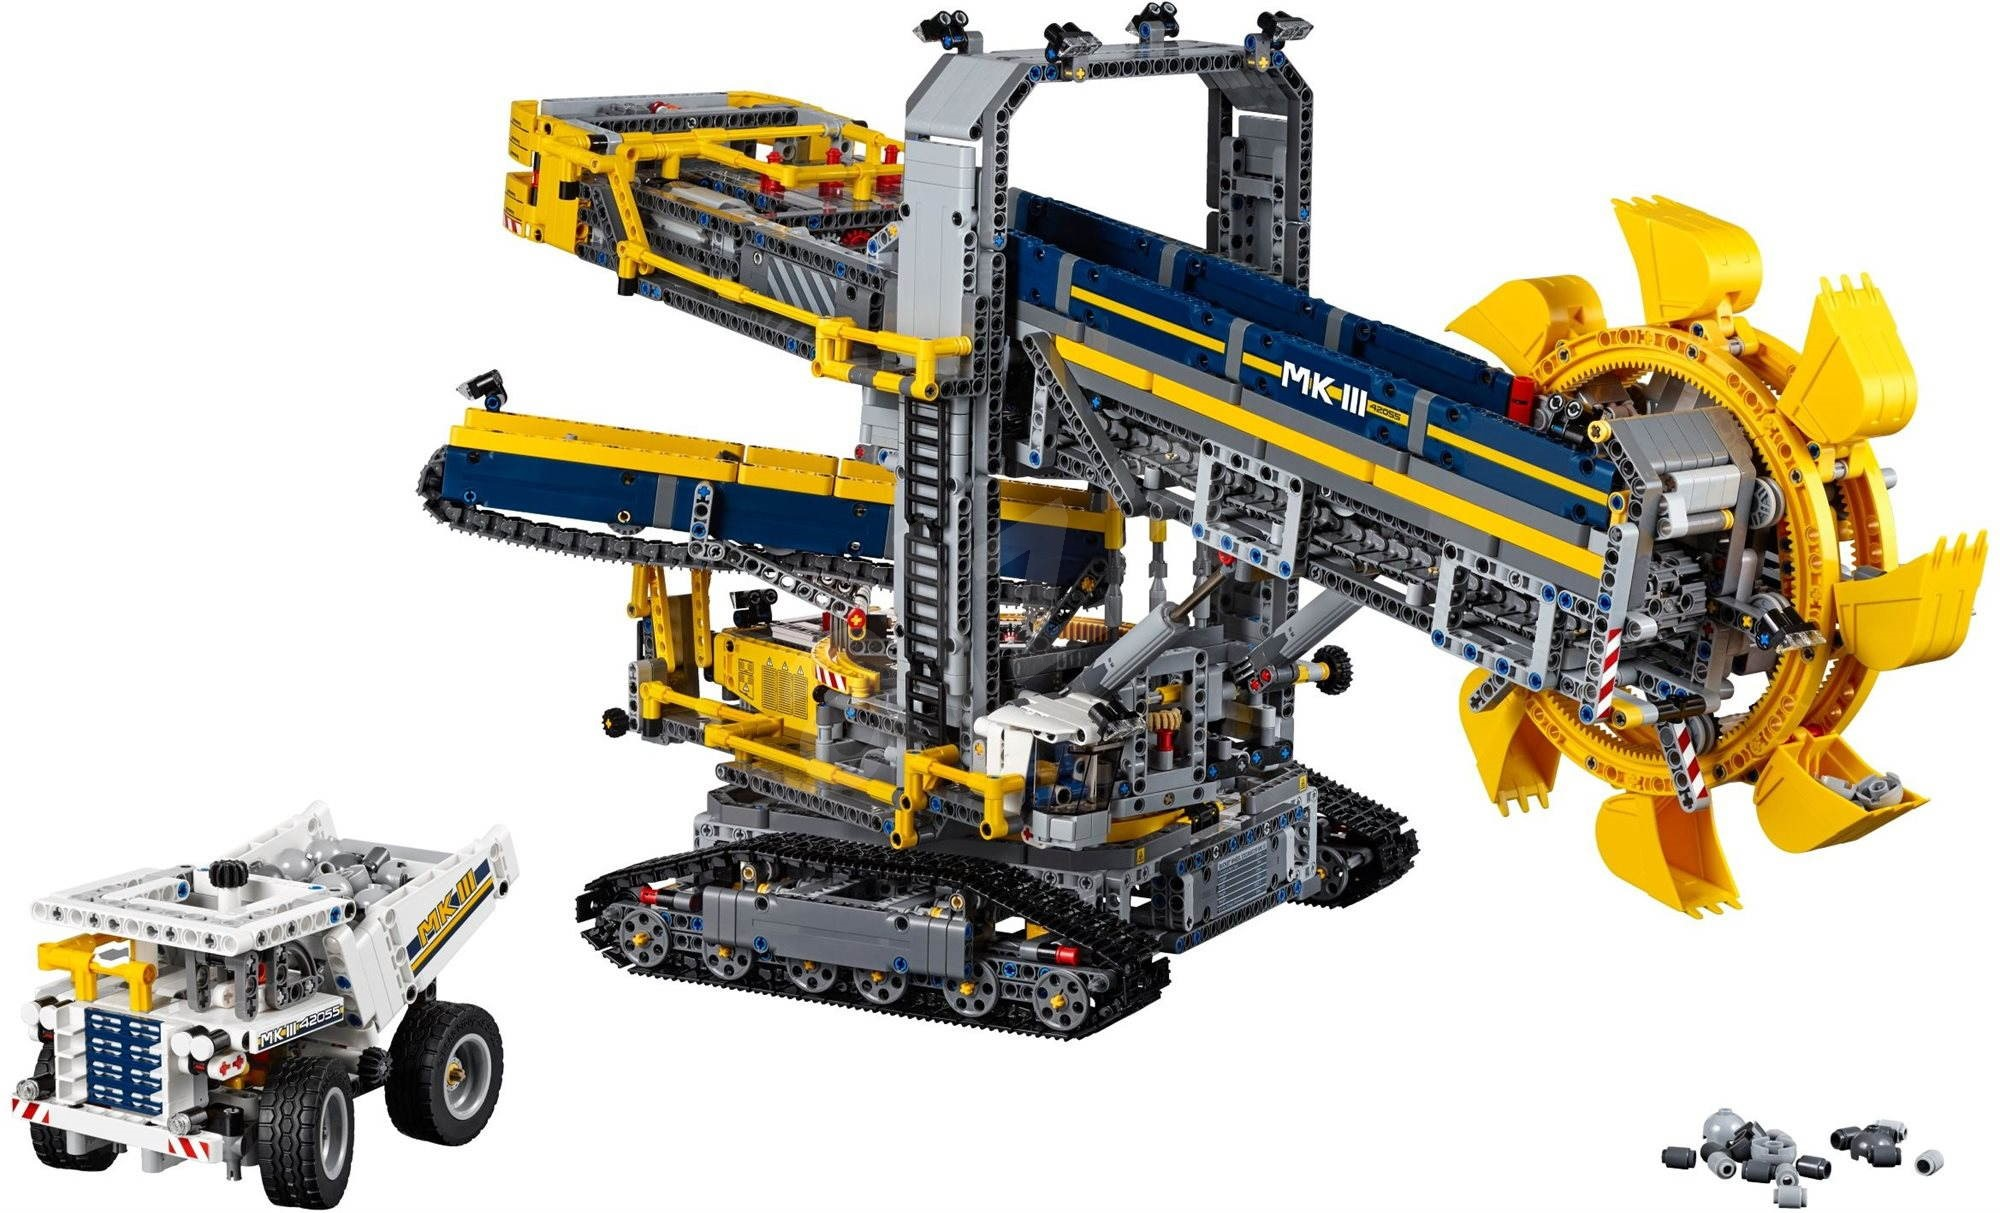
\includegraphics[width=13.5cm]{lego-technic.jpg}

Plastic connecting rods, shafts, pins, gears and similar parts. It's purpose
is to enable building more complex mechanical models than what is possible
with the more traditional "studded" LEGO blocks.

\subsection{LEGO Power Functions}

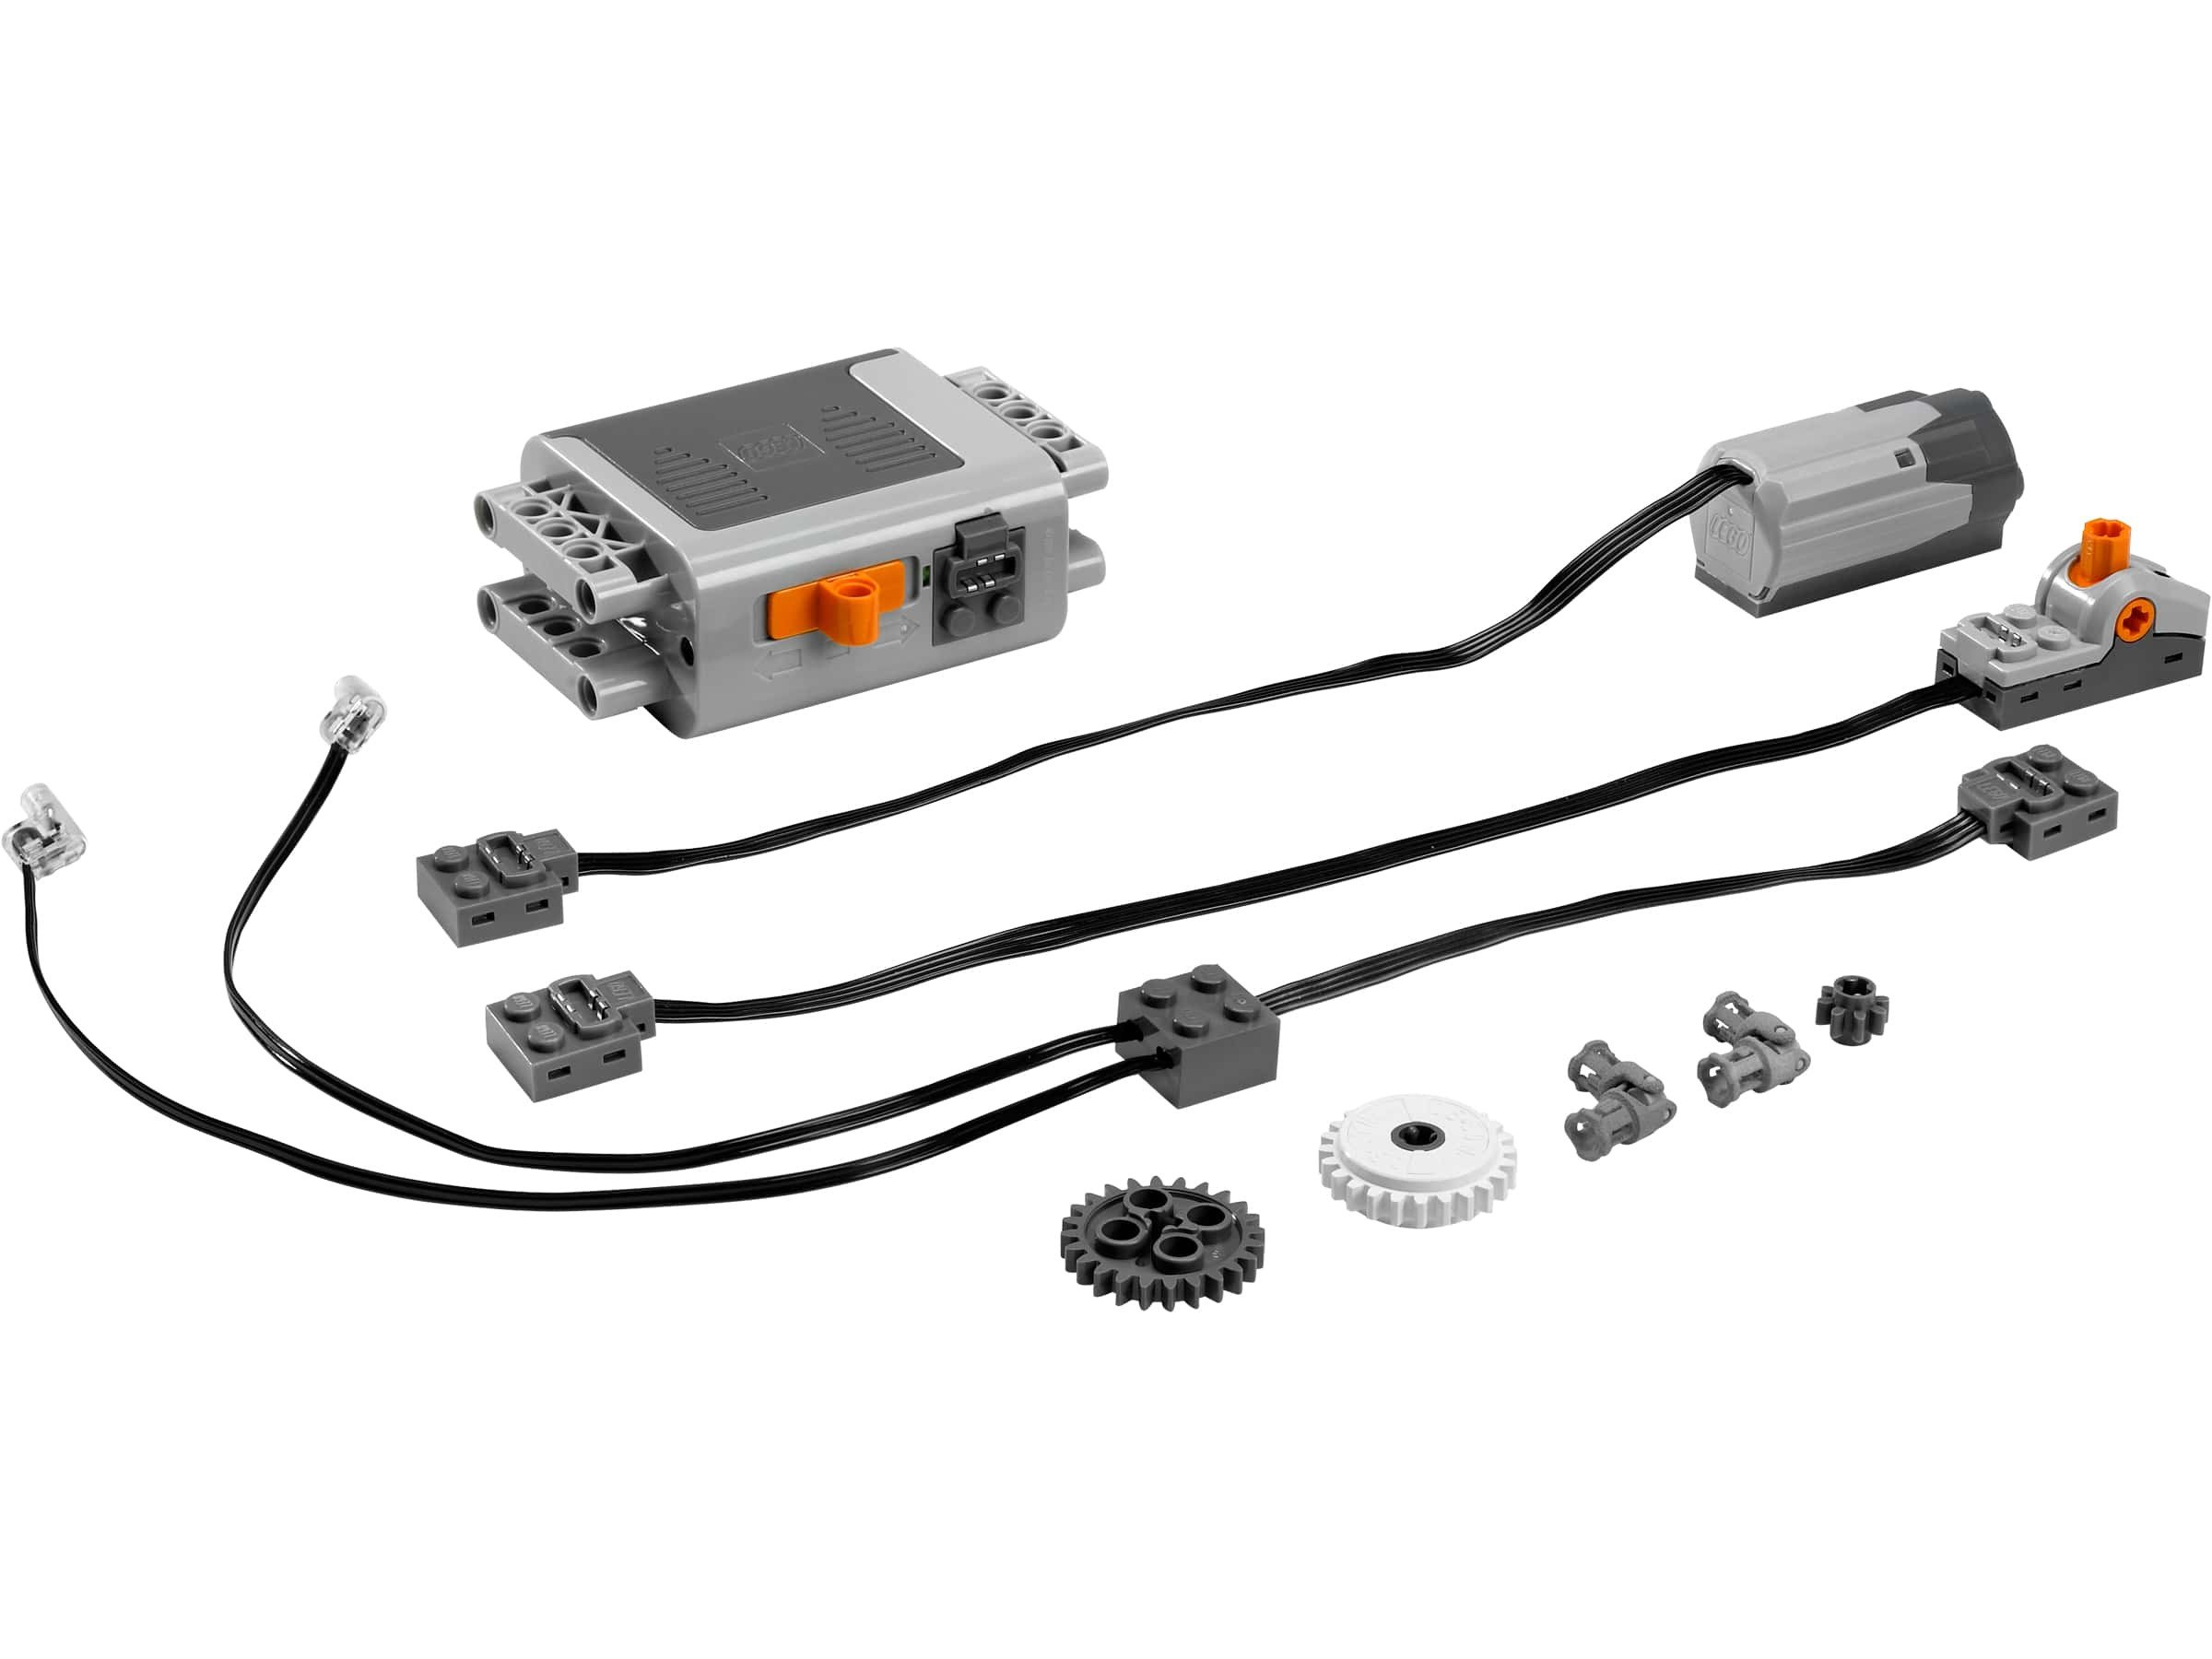
\includegraphics[width=13.5cm]{lego-power-functions.jpg}

Can be used with the LEGO Technic family, available from 2007. Engines, and
other accessories: lighting, battery box, rechargable battery, extension cable,
switch, remote controls. These can be used to turn manually operated Technic
models into battery operated toys.

\subsection{LEGO WeDo}

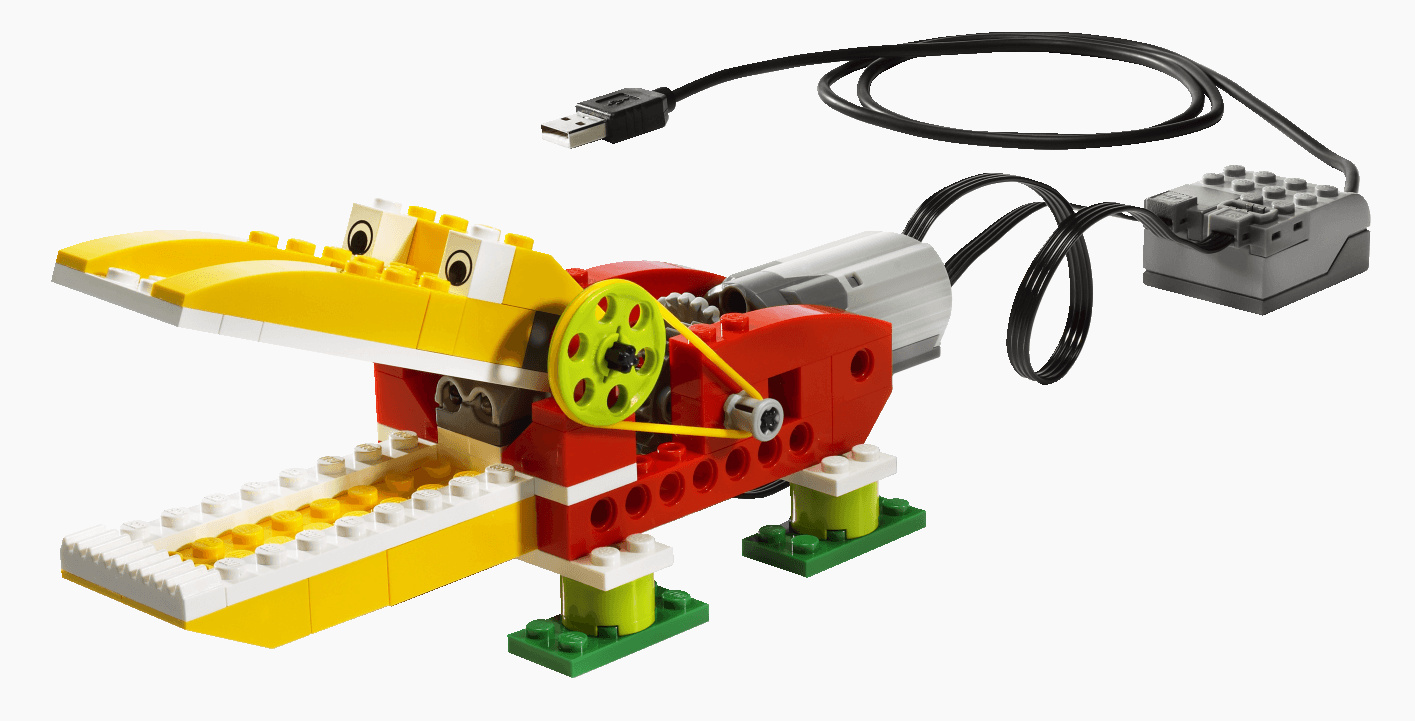
\includegraphics[width=13.5cm]{lego-wedo.jpg}

Central unit with USB connectivity and four connectors. Motor, tilt sensor,
proximity sensor.

\subsection{LEGO WeDo 2.0}

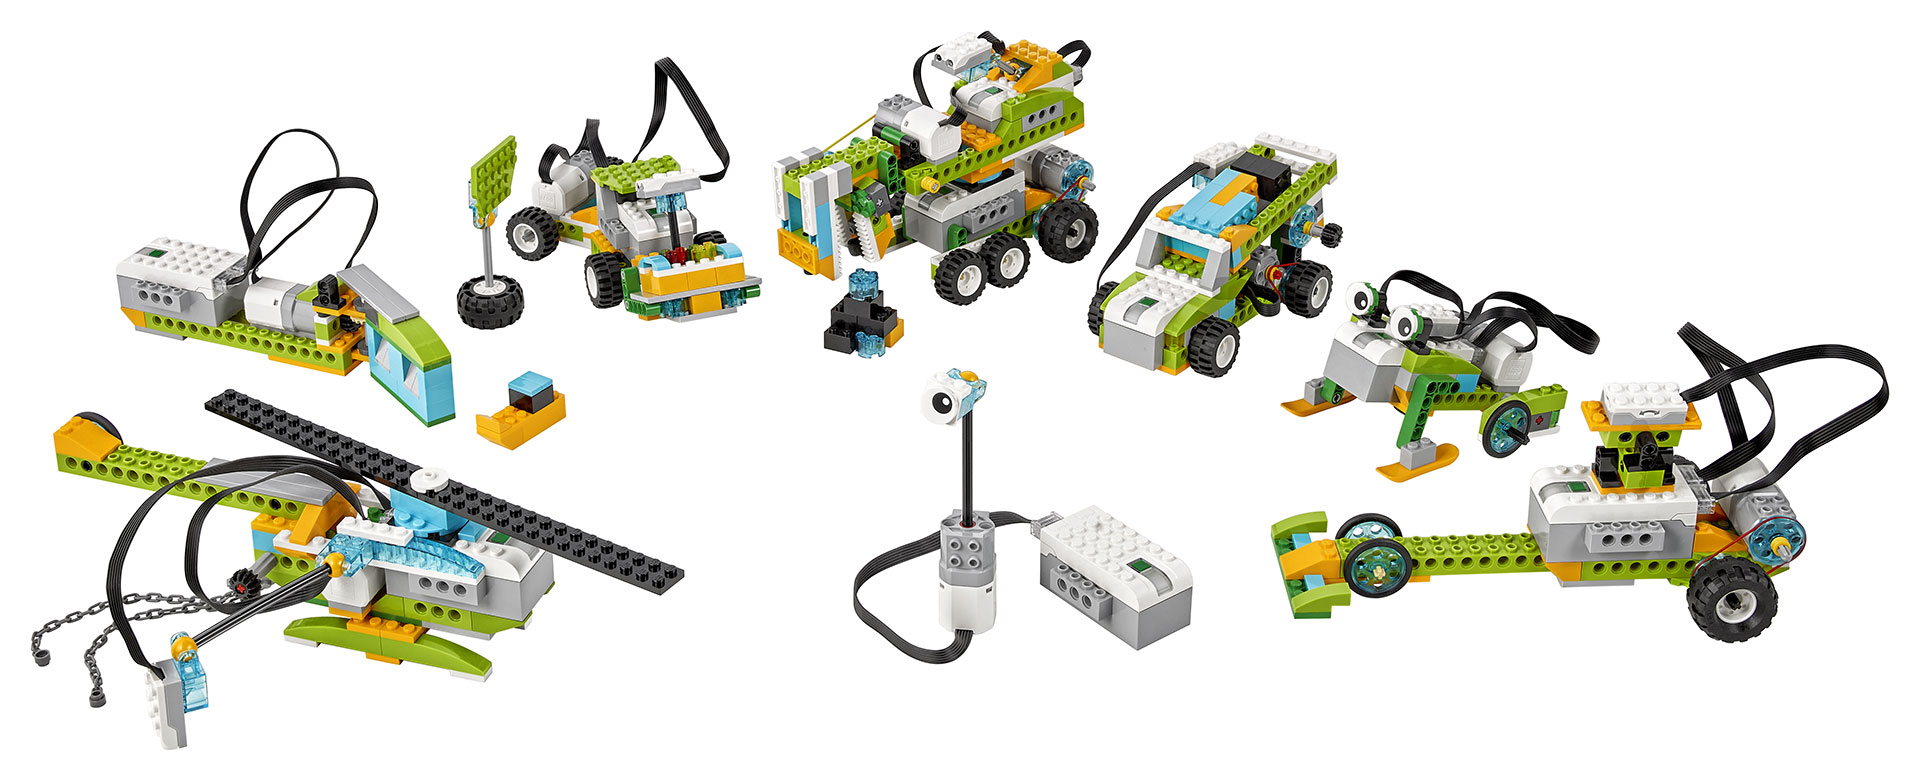
\includegraphics[width=13.5cm]{lego-wedo-2.jpg}

The next version of the WeDo set with different connectors and a smarter,
Bluetooth capable central unit.

\subsection{LEGO Boost}

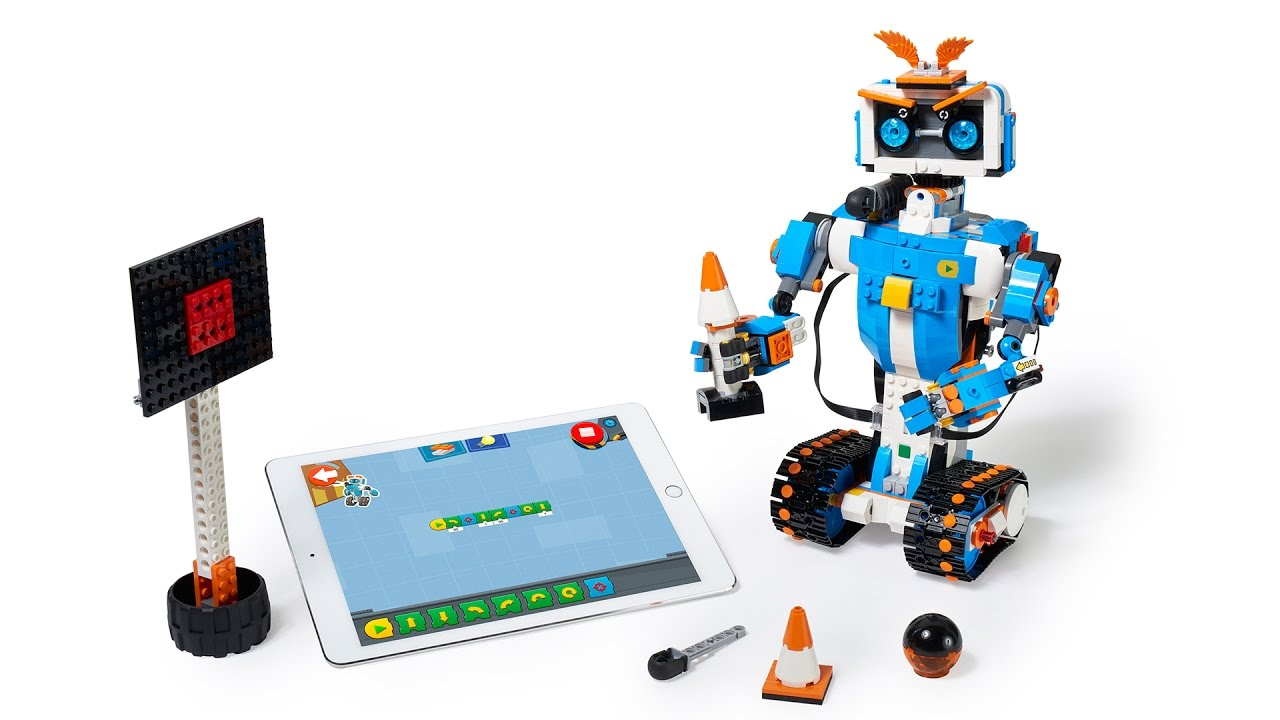
\includegraphics[width=13.5cm]{lego-boost.jpg}

Robotic building set with parts similar to WeDo 2.0, with identical connectors.
While the WeDo line of products are primarily for education purposes, the Boost
line is mainly for play.

\subsection{LEGO MindStorms EV3}

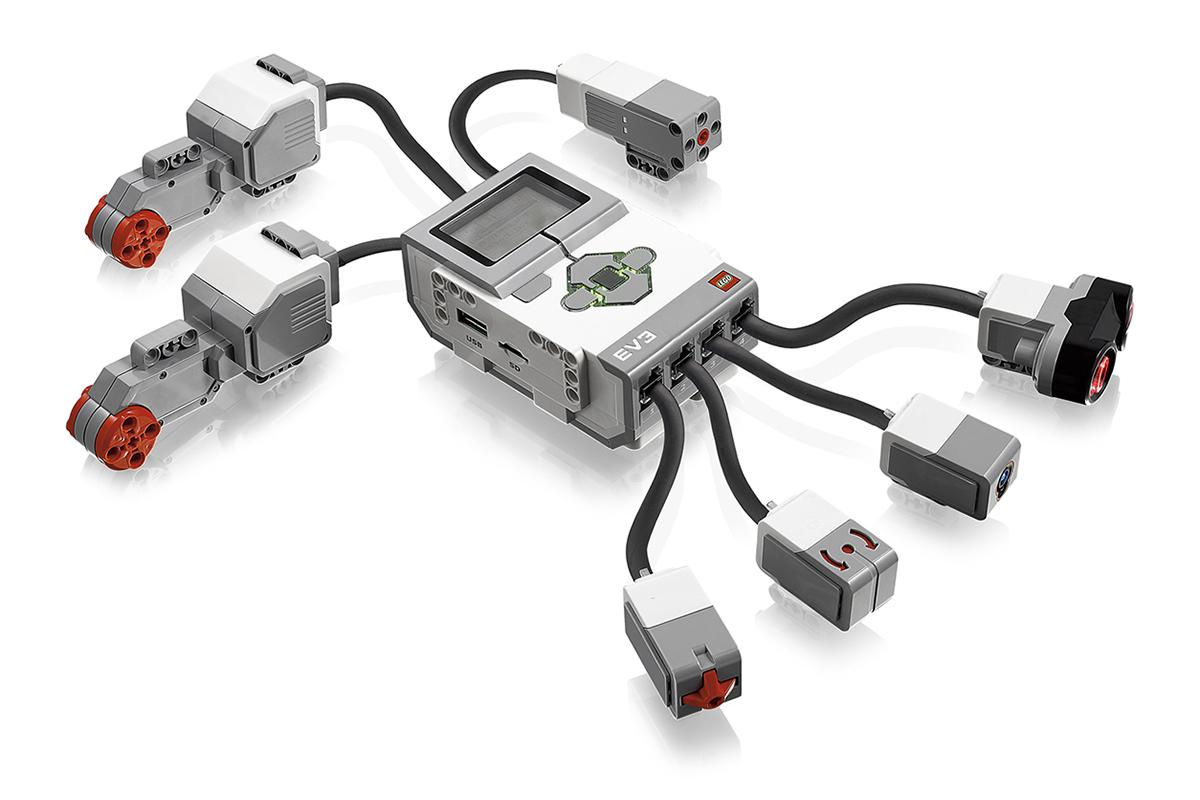
\includegraphics[width=13.5cm]{lego-mindstorms-ev3.jpg}

Robotic building set with central unit, motors, sensors, and cables. The set
uses connectors \emph{similar} to RJ12 (6P6C modular).

\subsection{LEGO MindStorms NXT 1.0 and 2.0}

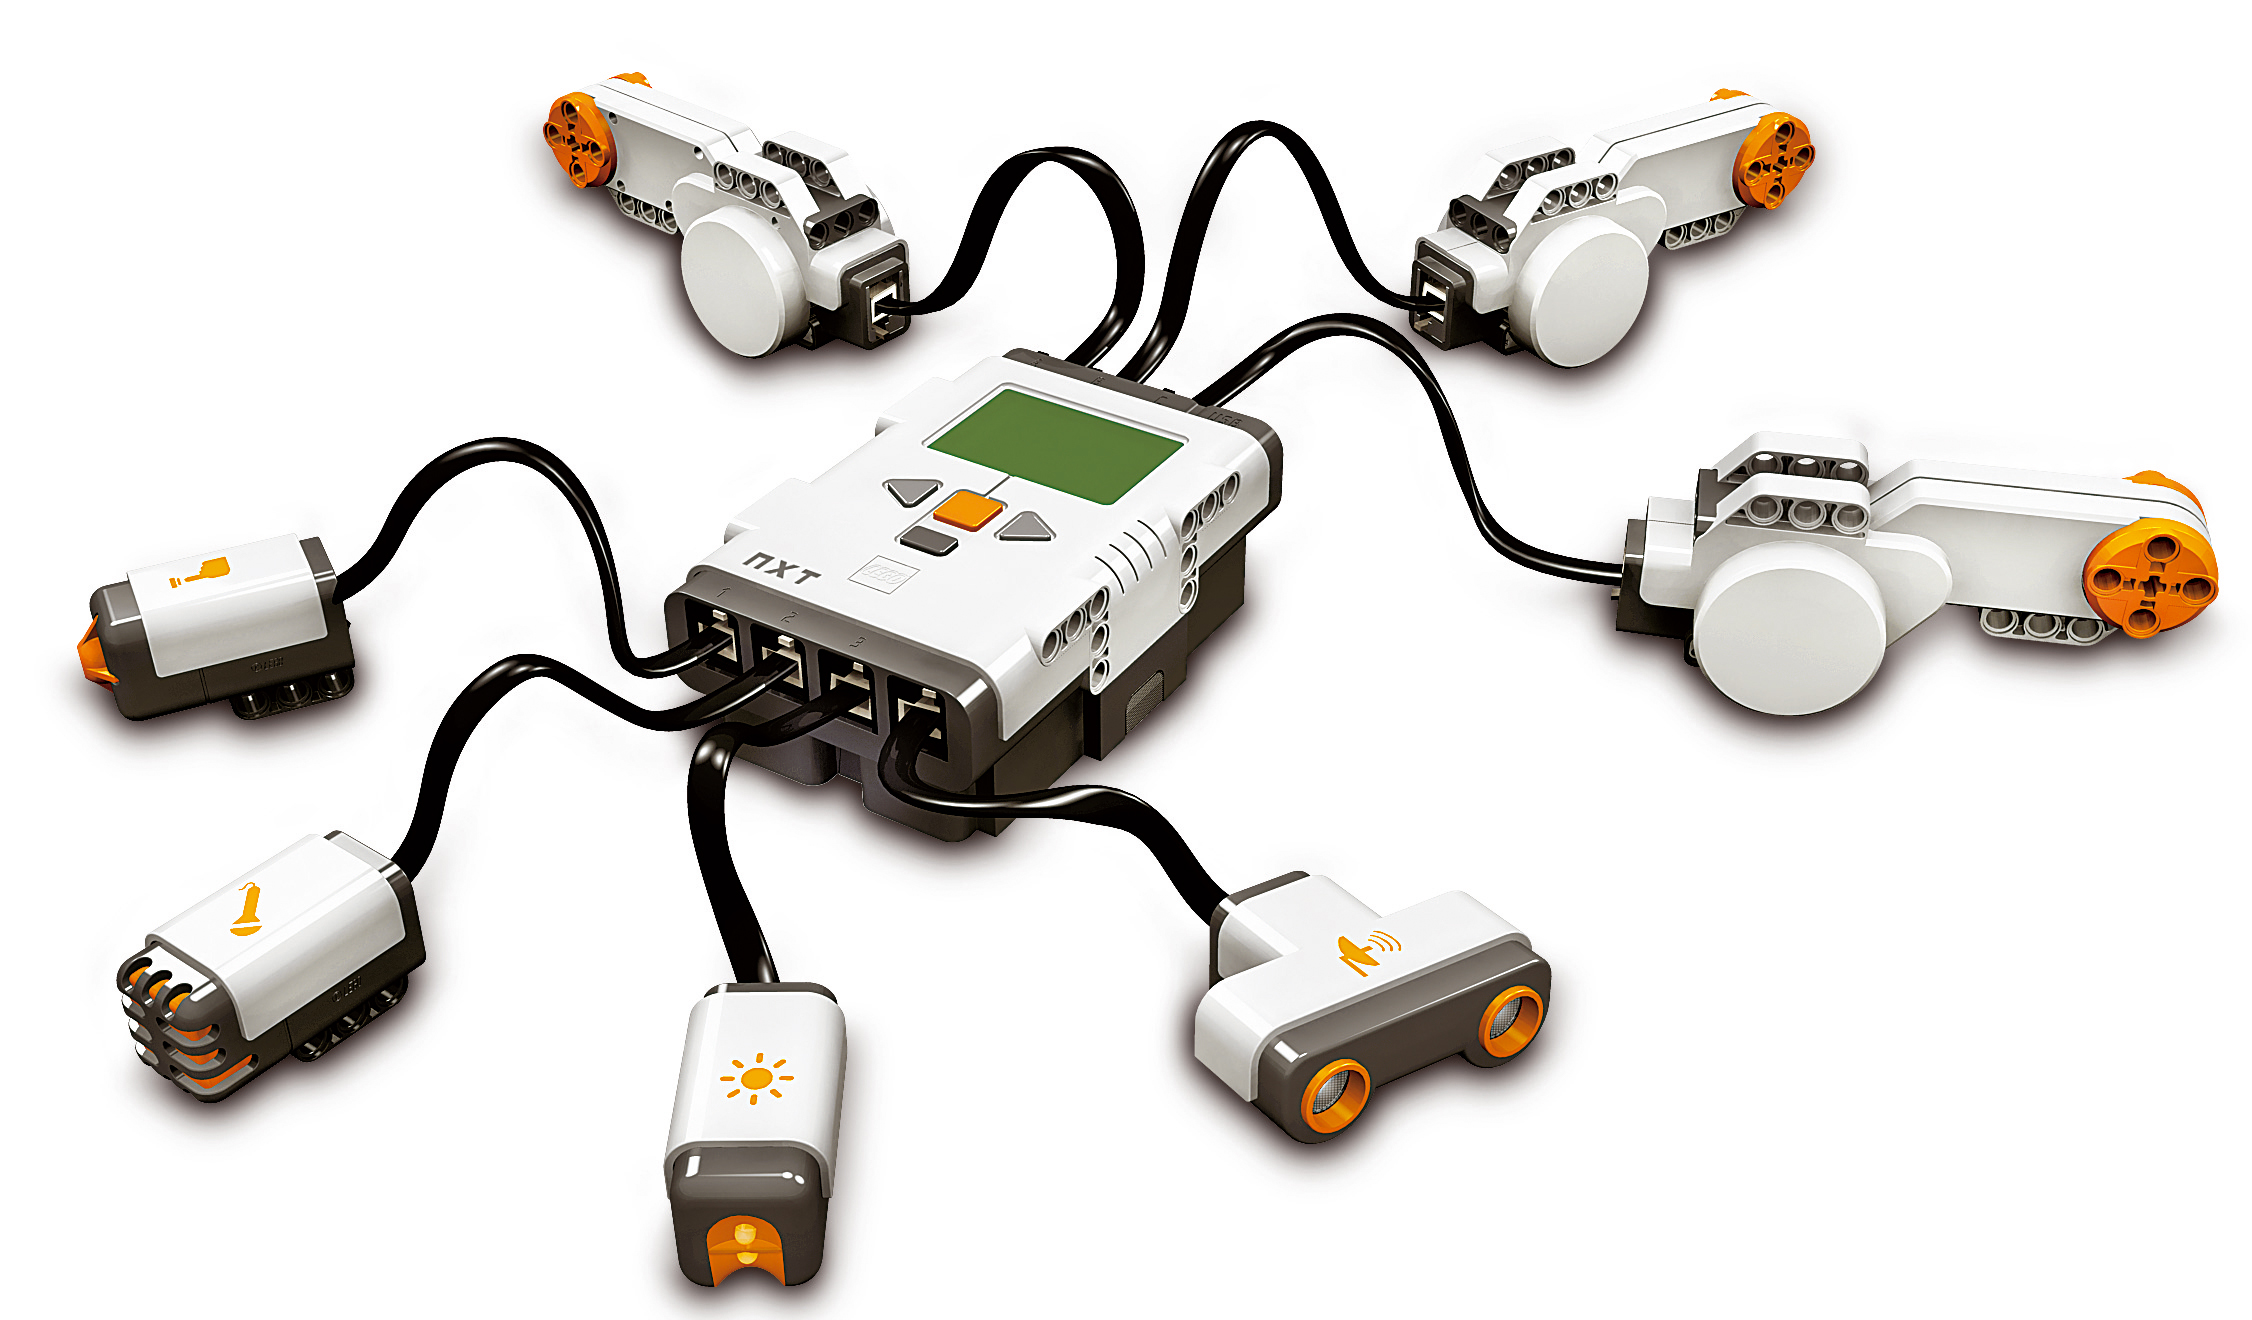
\includegraphics[width=13.5cm]{lego-mindstorms-nxt.jpg}

Robotic building set similar to EV3.

\section{Role and operation the SBrick Plus adapters}

\emph{SBrick} can only be used with Power Functions motors, servos and lights.
Although WeDo sensors can be physically attached to SBrick, they cannot be
used, since SBrick can't read the voltage they output.

\emph{SBrick Plus} can measure voltage, so it can be used with WeDo sensors.

The role of the adapters is to connect certain LEGO EV3/NXT and WeDo2 motors
and sensors physically, electricly and logically.

Although the SBrick can attach to any adapter, it's only useful to attach motor
adapters to it. Accidentally connecting sensor adapters to an SBrick should
never cause damage to the sensor nor to the SBrick.

The motor and sensor adapters are electronically different, so connecting
motors and sensors must be done with different adapters.

The EV3/NXT and WeDo 2 connectors are different, so they also need different
adapters.

\section{Adapter parts}

\subsection{Populated sensor adapter circuit}

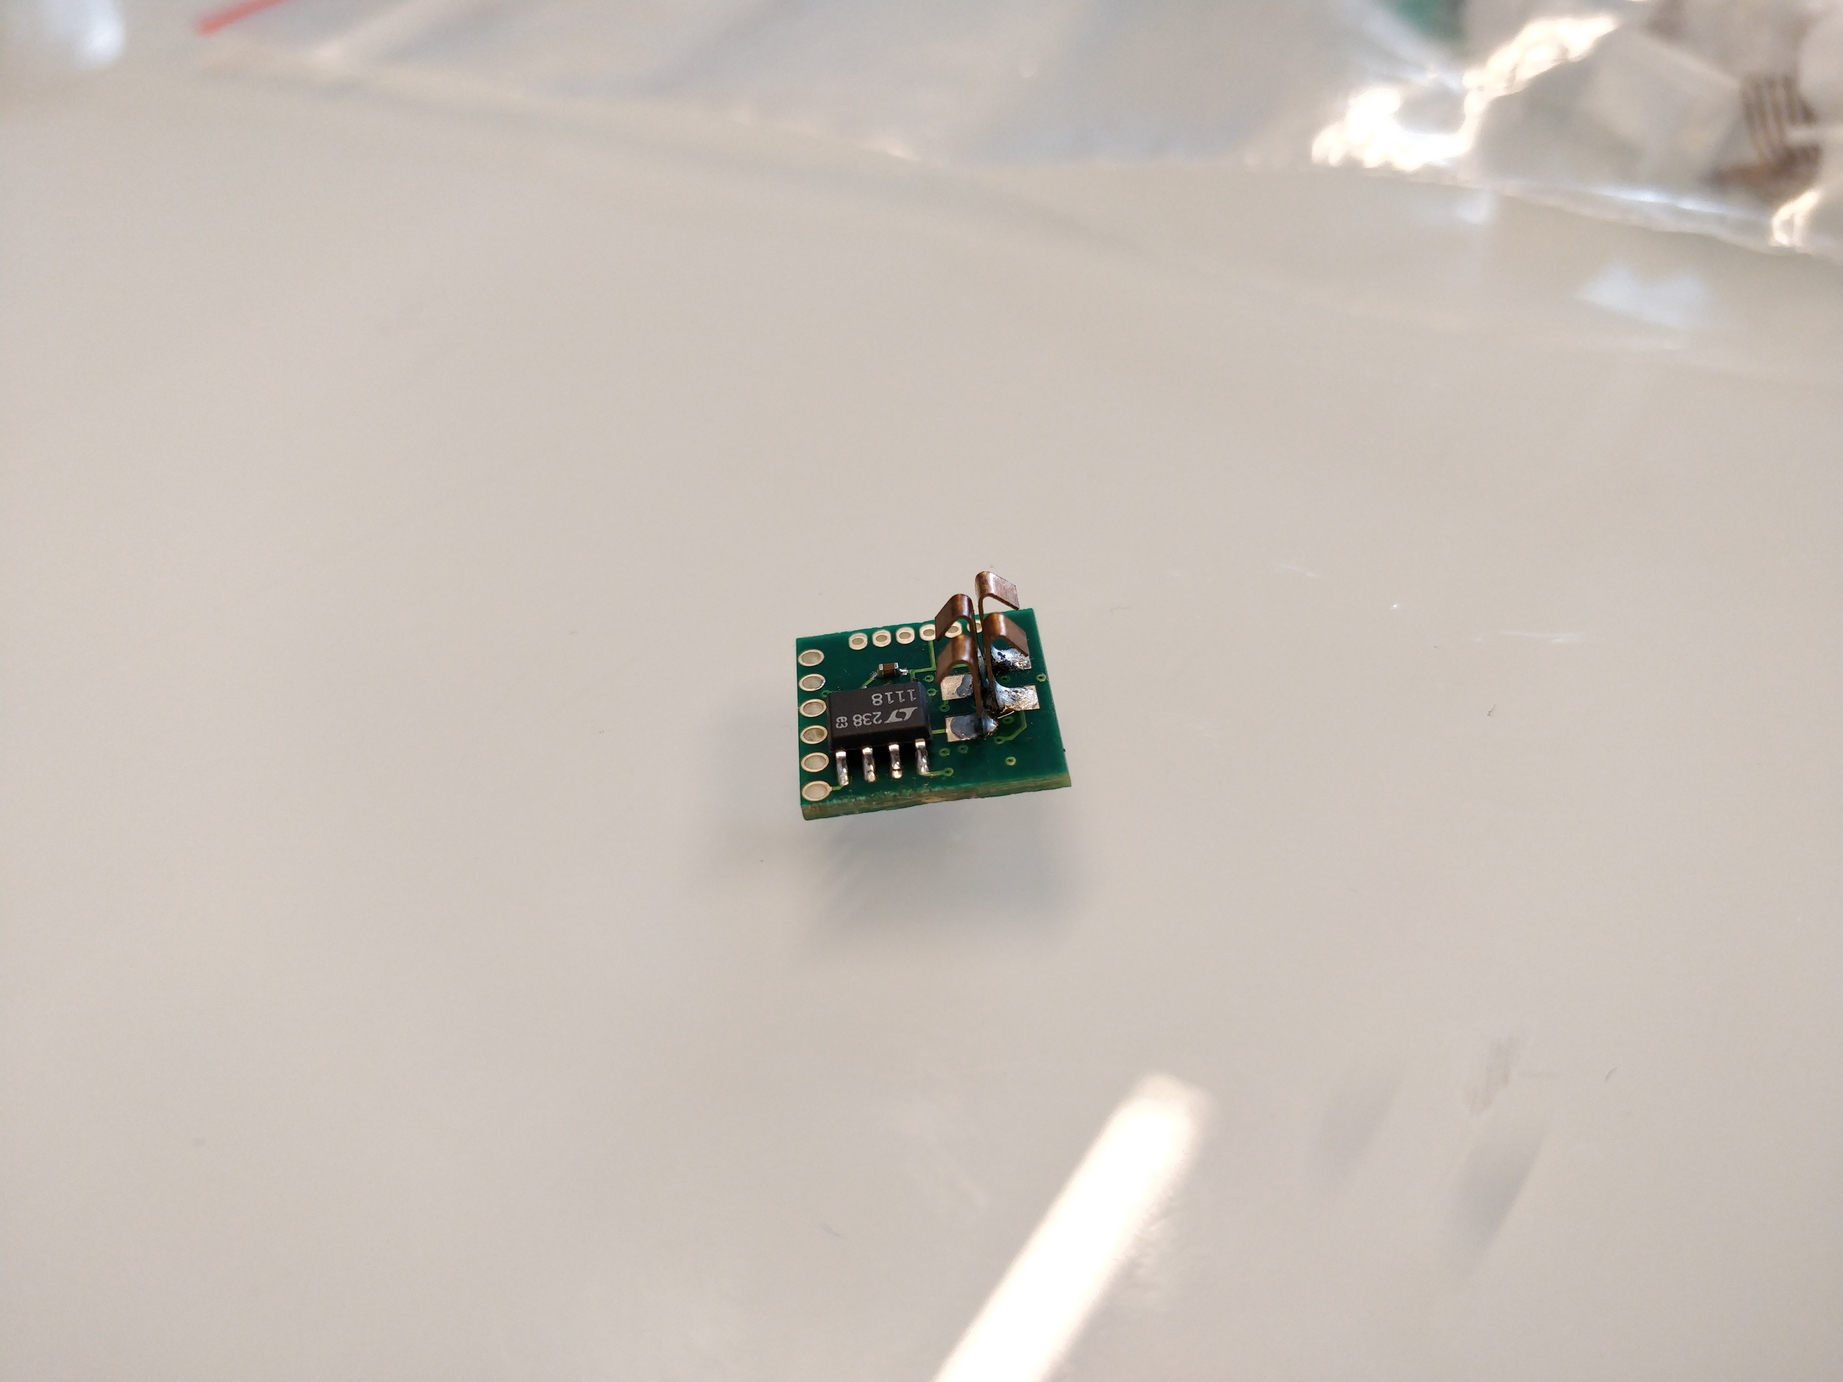
\includegraphics[width=13.5cm]{sensor-populated-circuit.jpg}

\subsection{Populated motor adapter}

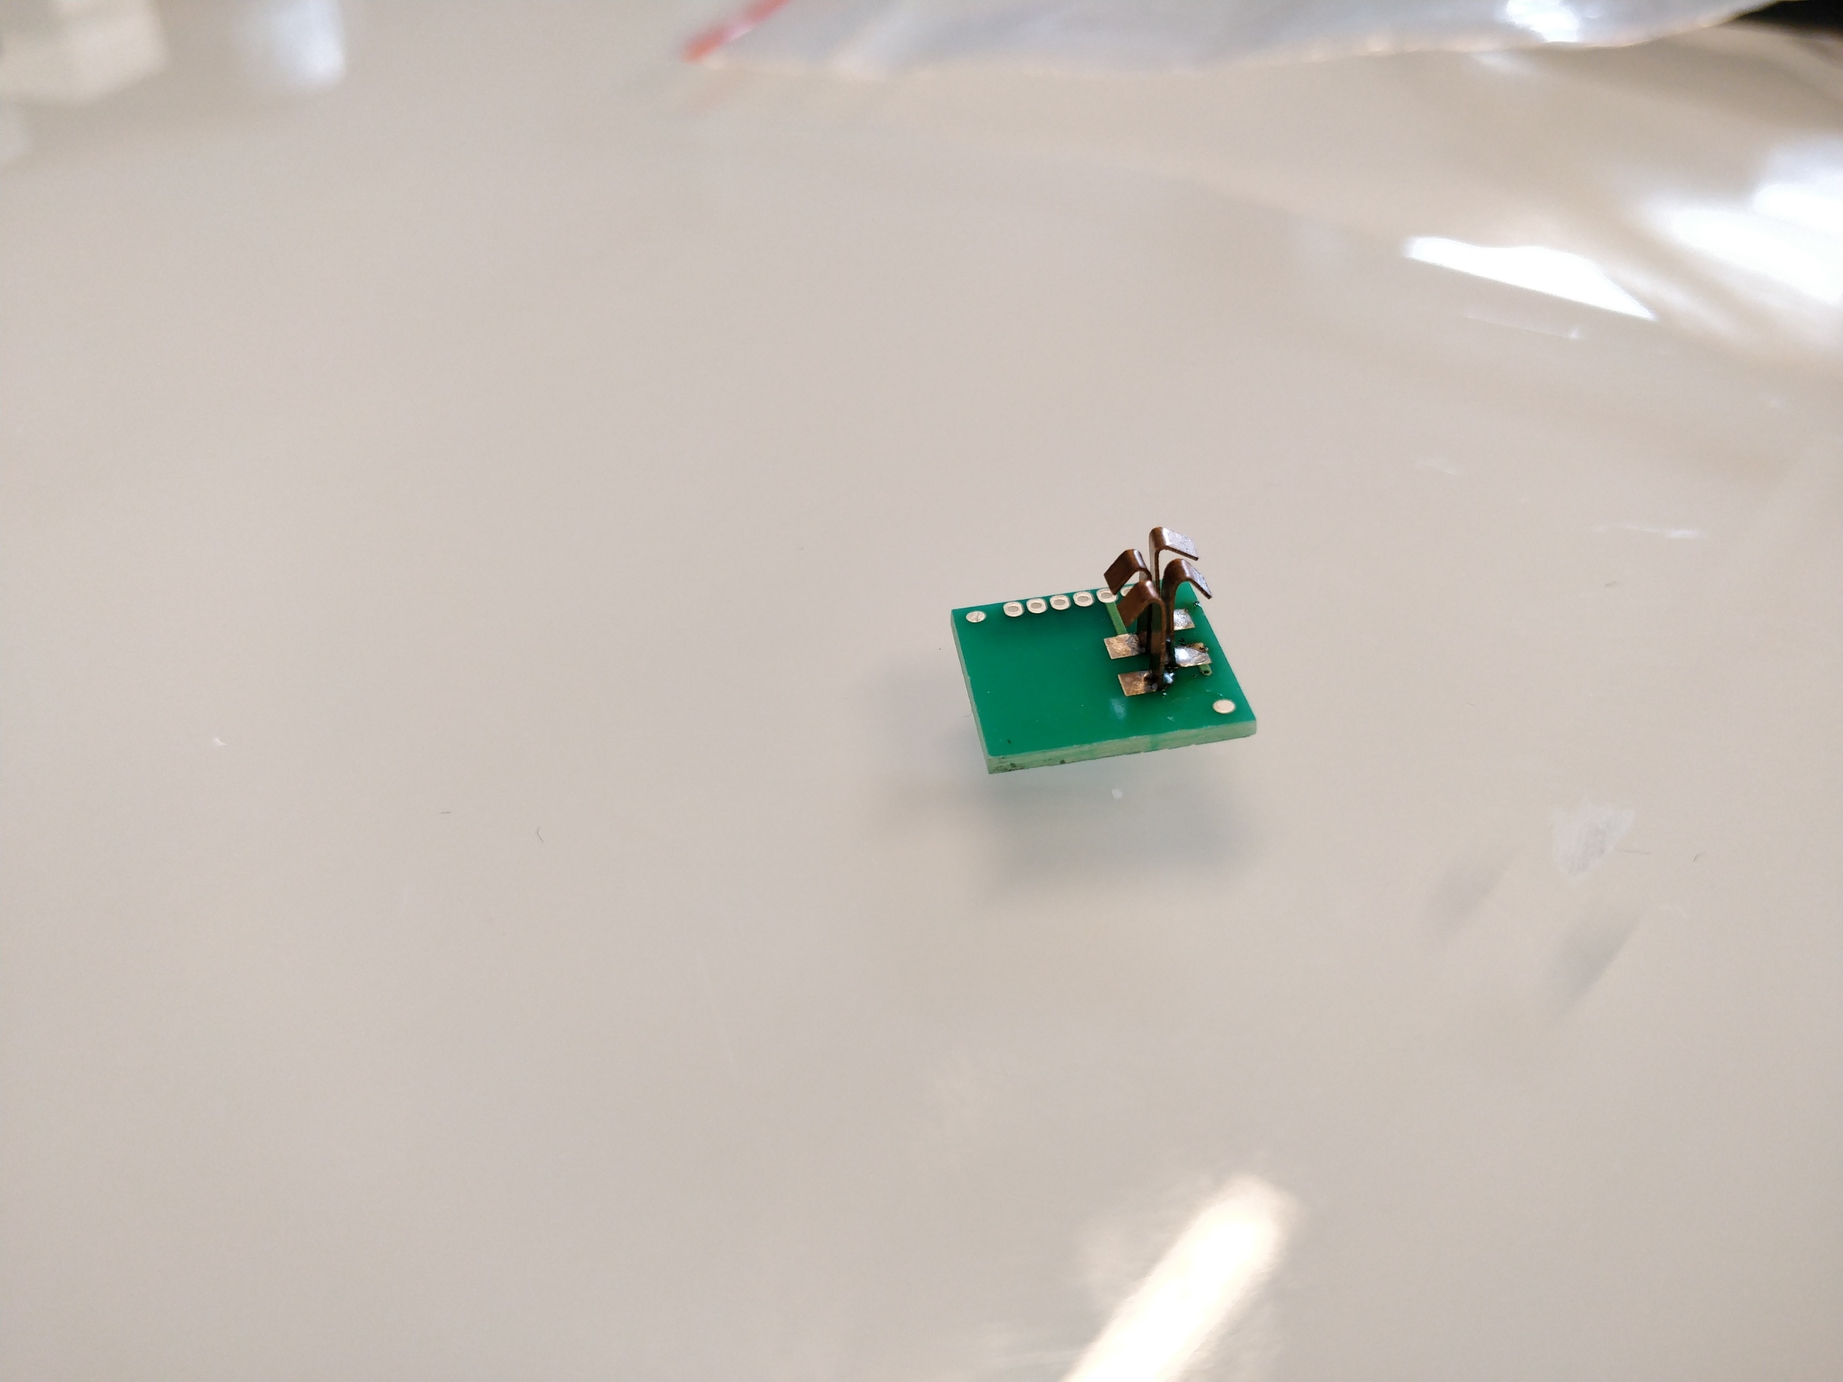
\includegraphics[width=13.5cm]{motor-populated-circuit.jpg}

\subsection{Wedo 2 adapter pins}

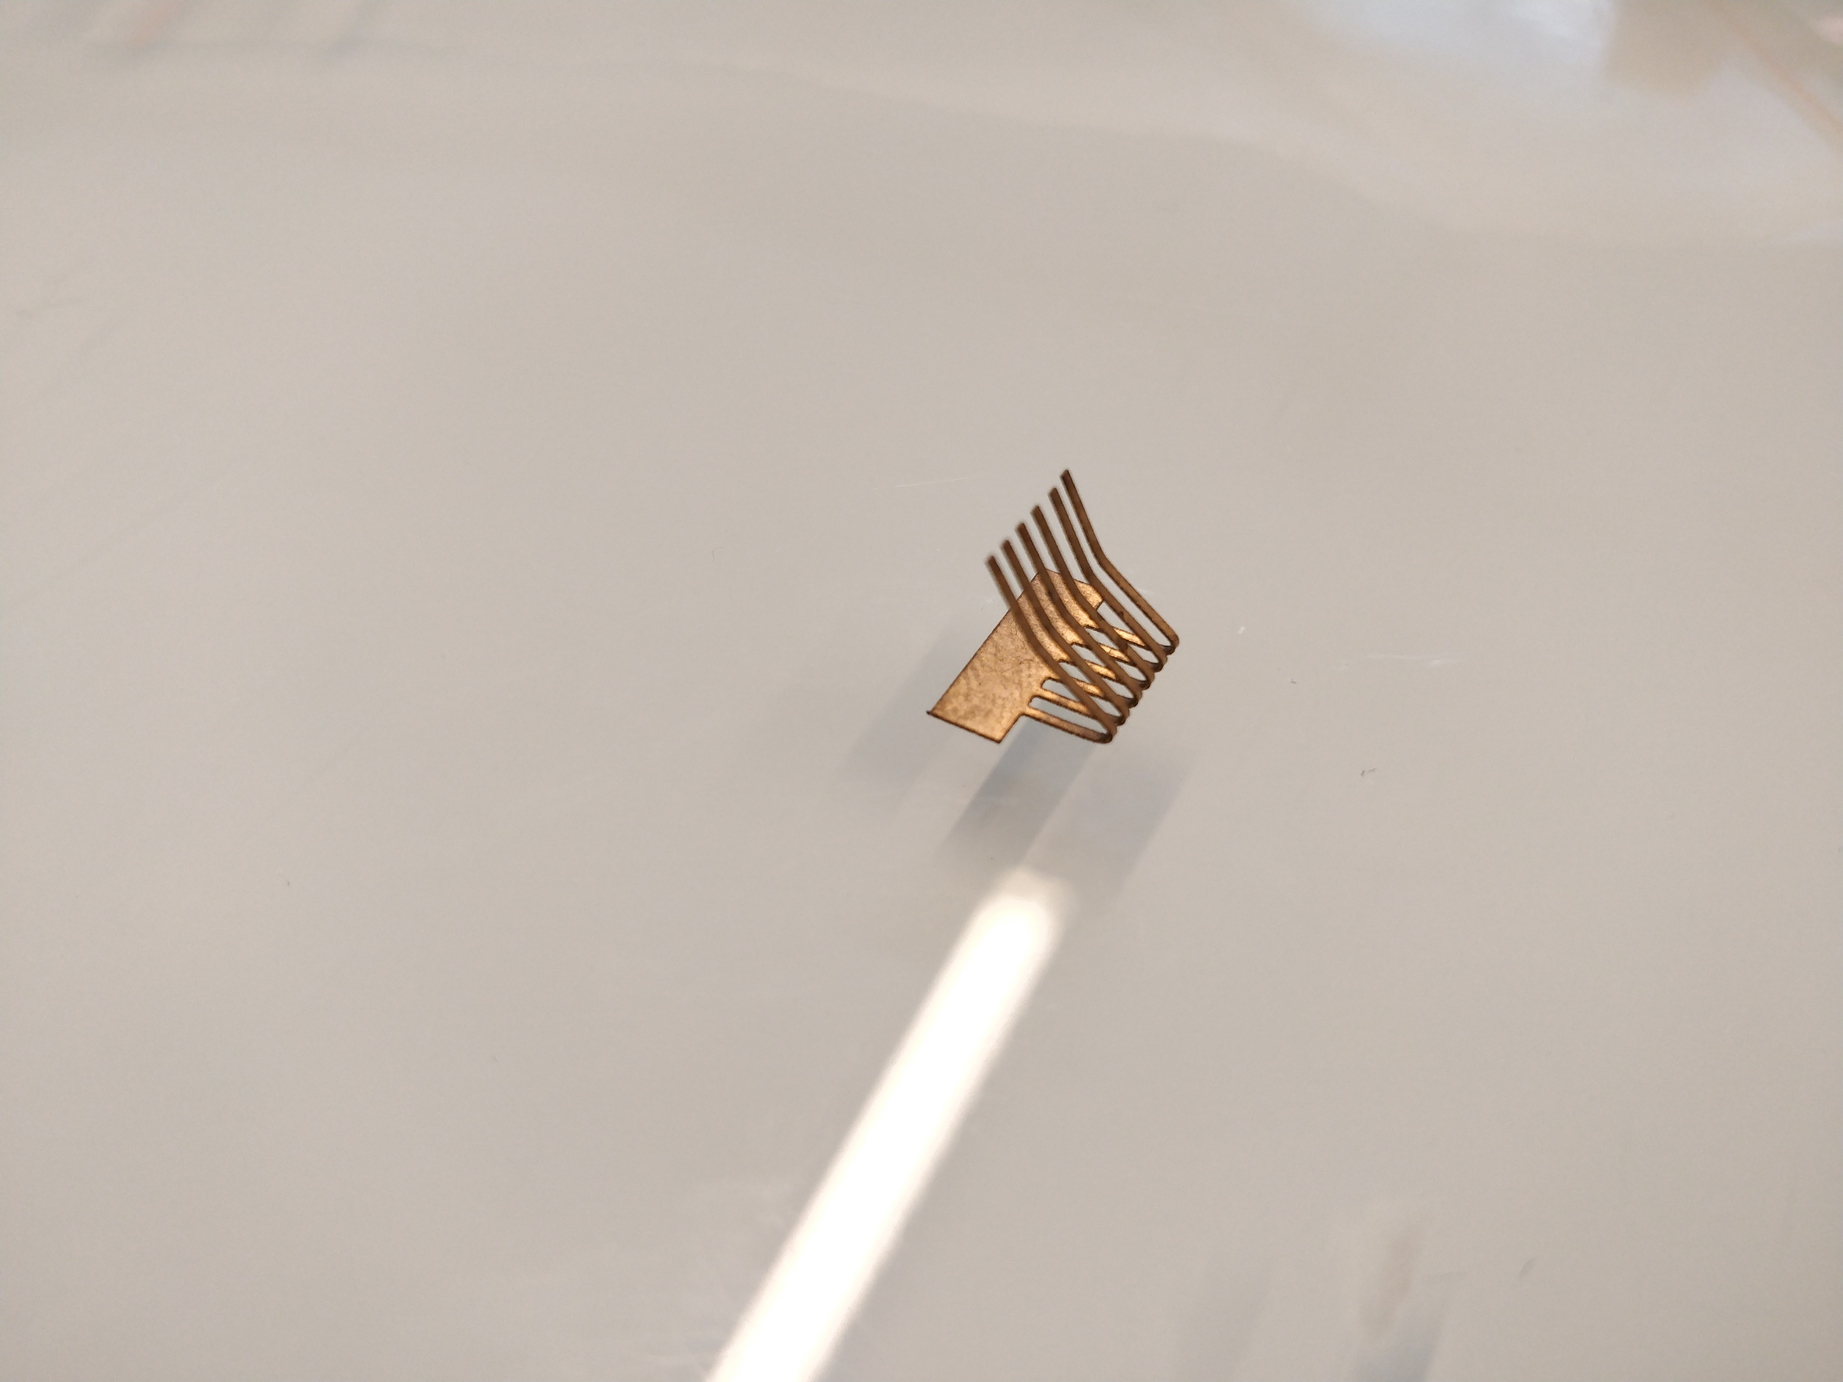
\includegraphics[width=13.5cm]{wedo2-pins.jpg}

\subsection{Power Functions pins}

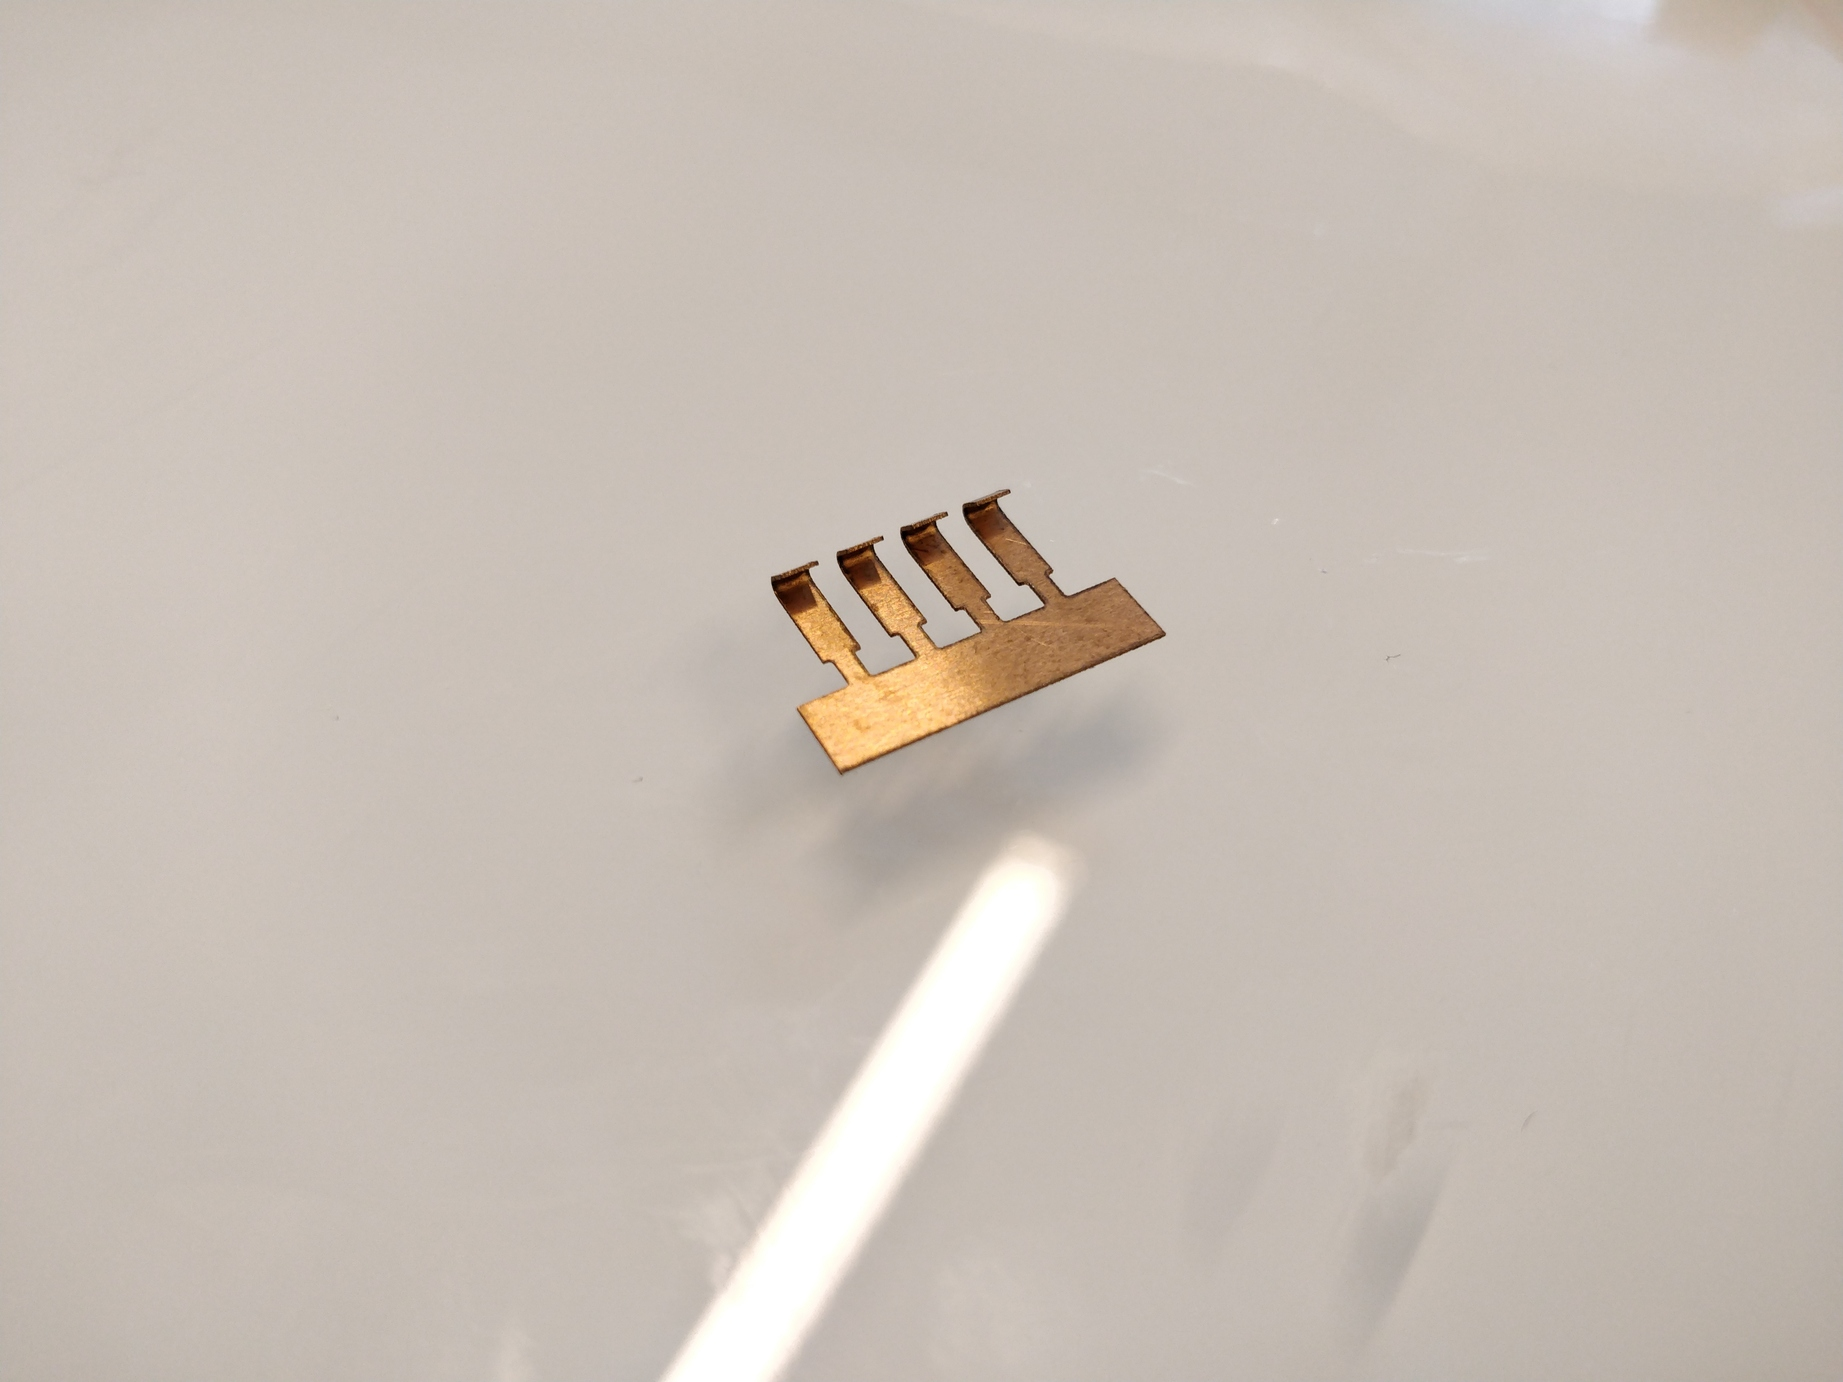
\includegraphics[width=13.5cm]{power-functions-pins.jpg}

\subsection{Wedo 2 motor adapter case insert}

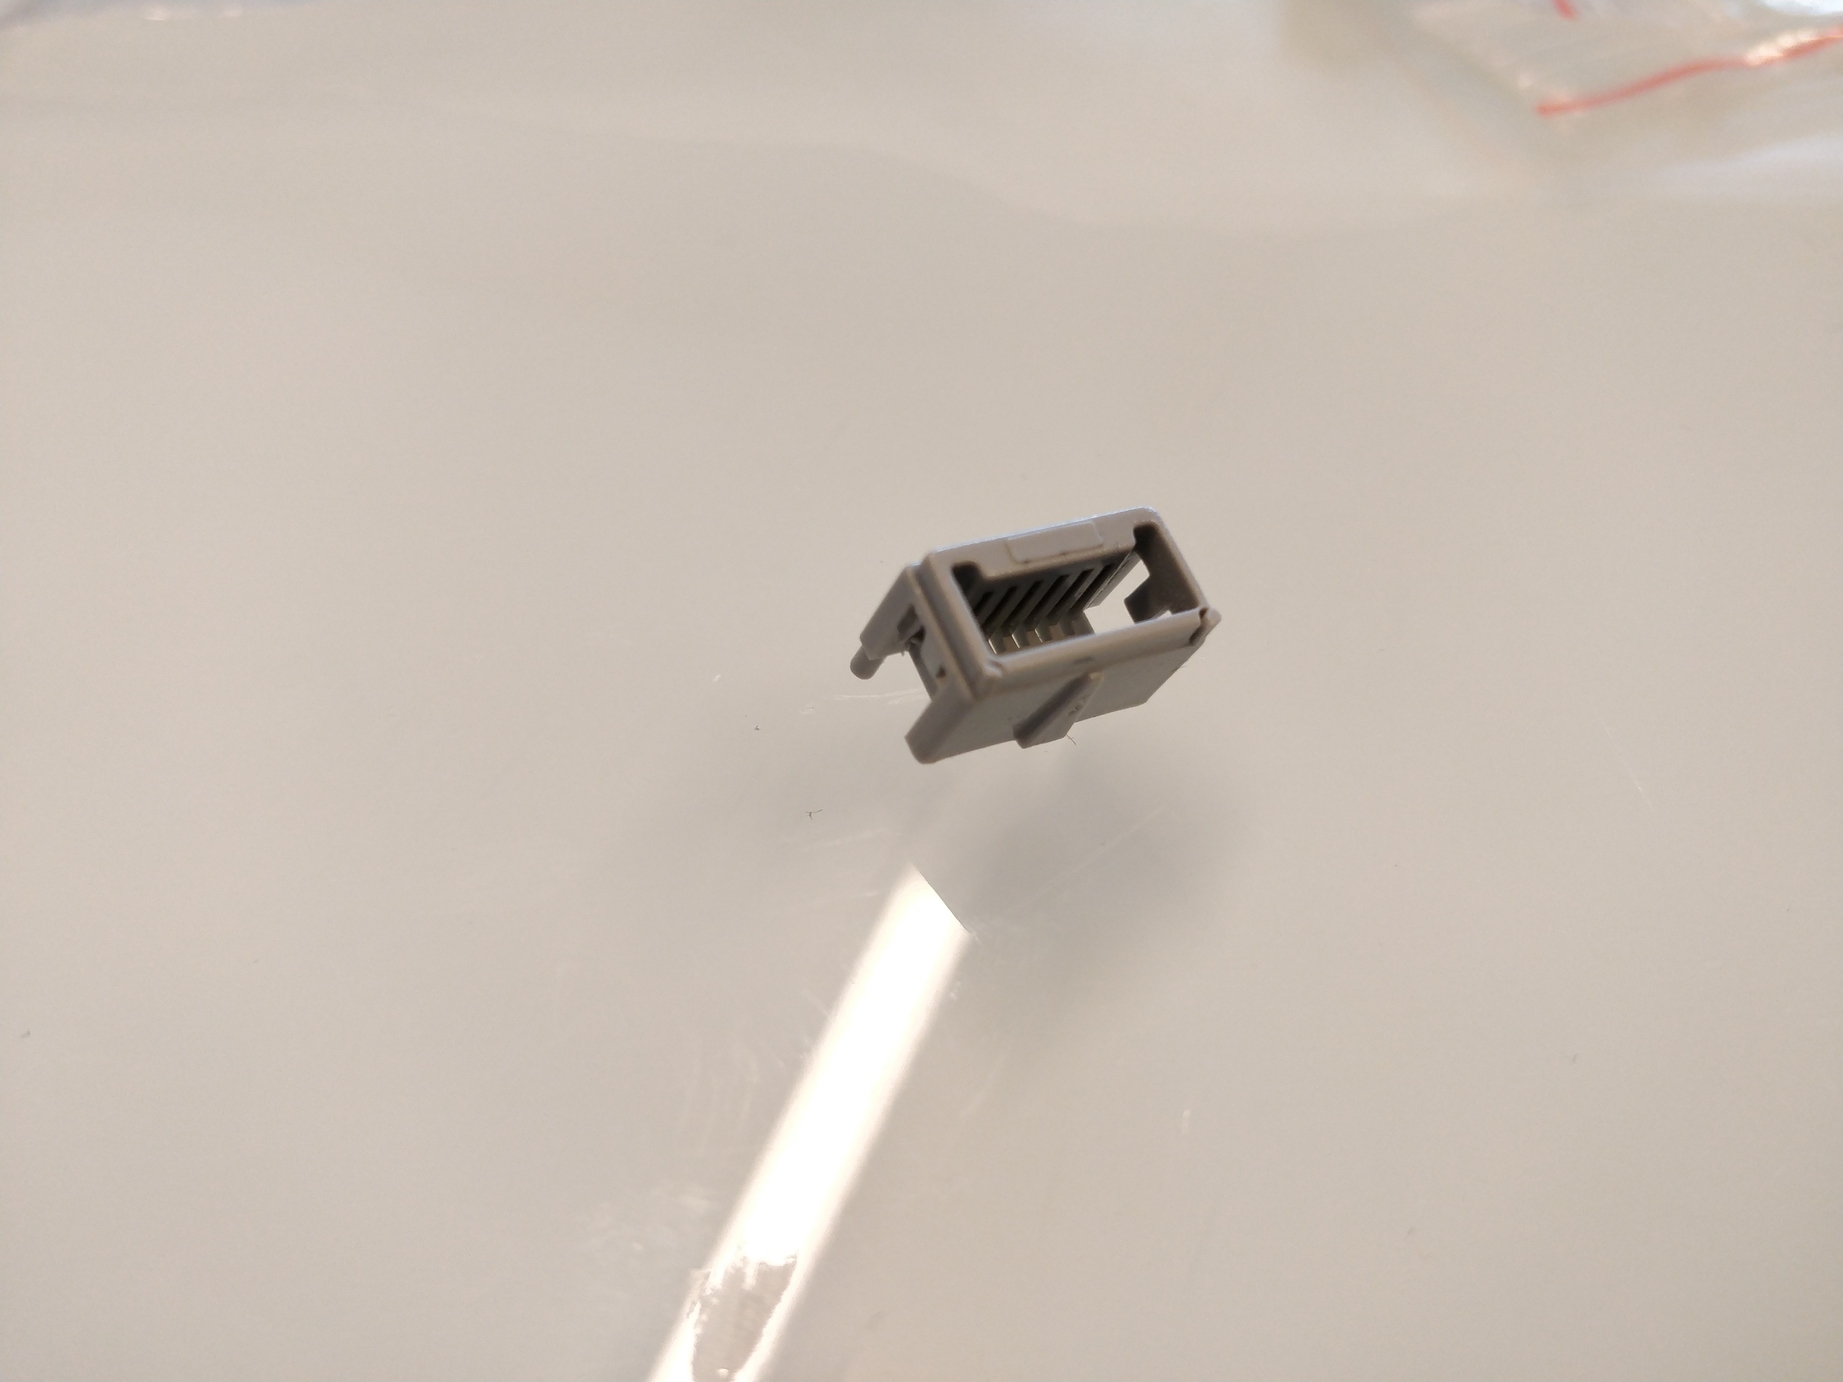
\includegraphics[width=13.5cm]{wedo2-motor-plastic-insert.jpg}

\subsection{EV3 motor adapter case insert}

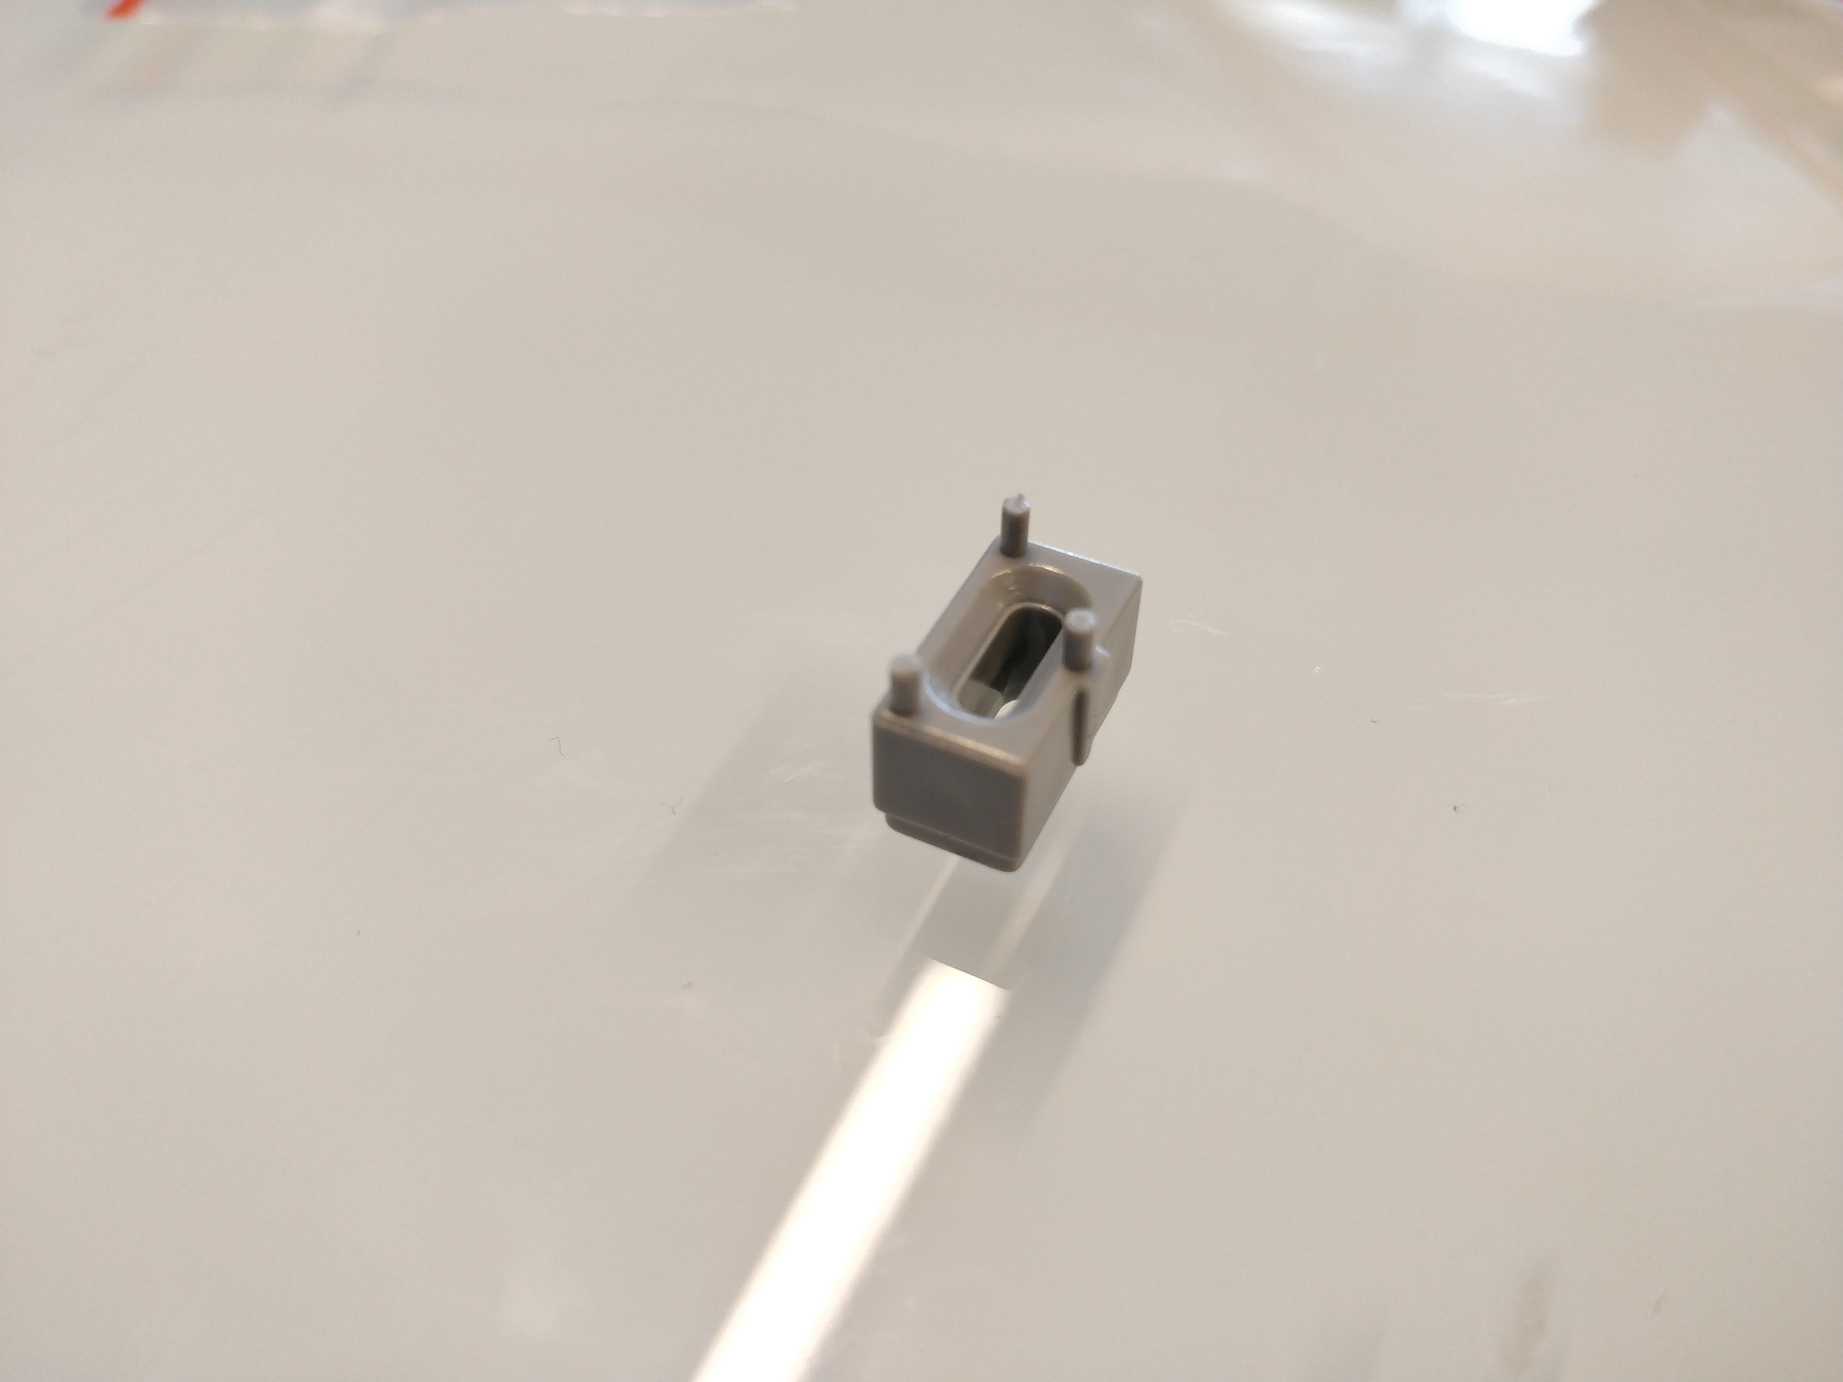
\includegraphics[width=13.5cm]{ev3-motor-plastic-insert.jpg}

\subsection{Motor adapter case top part}

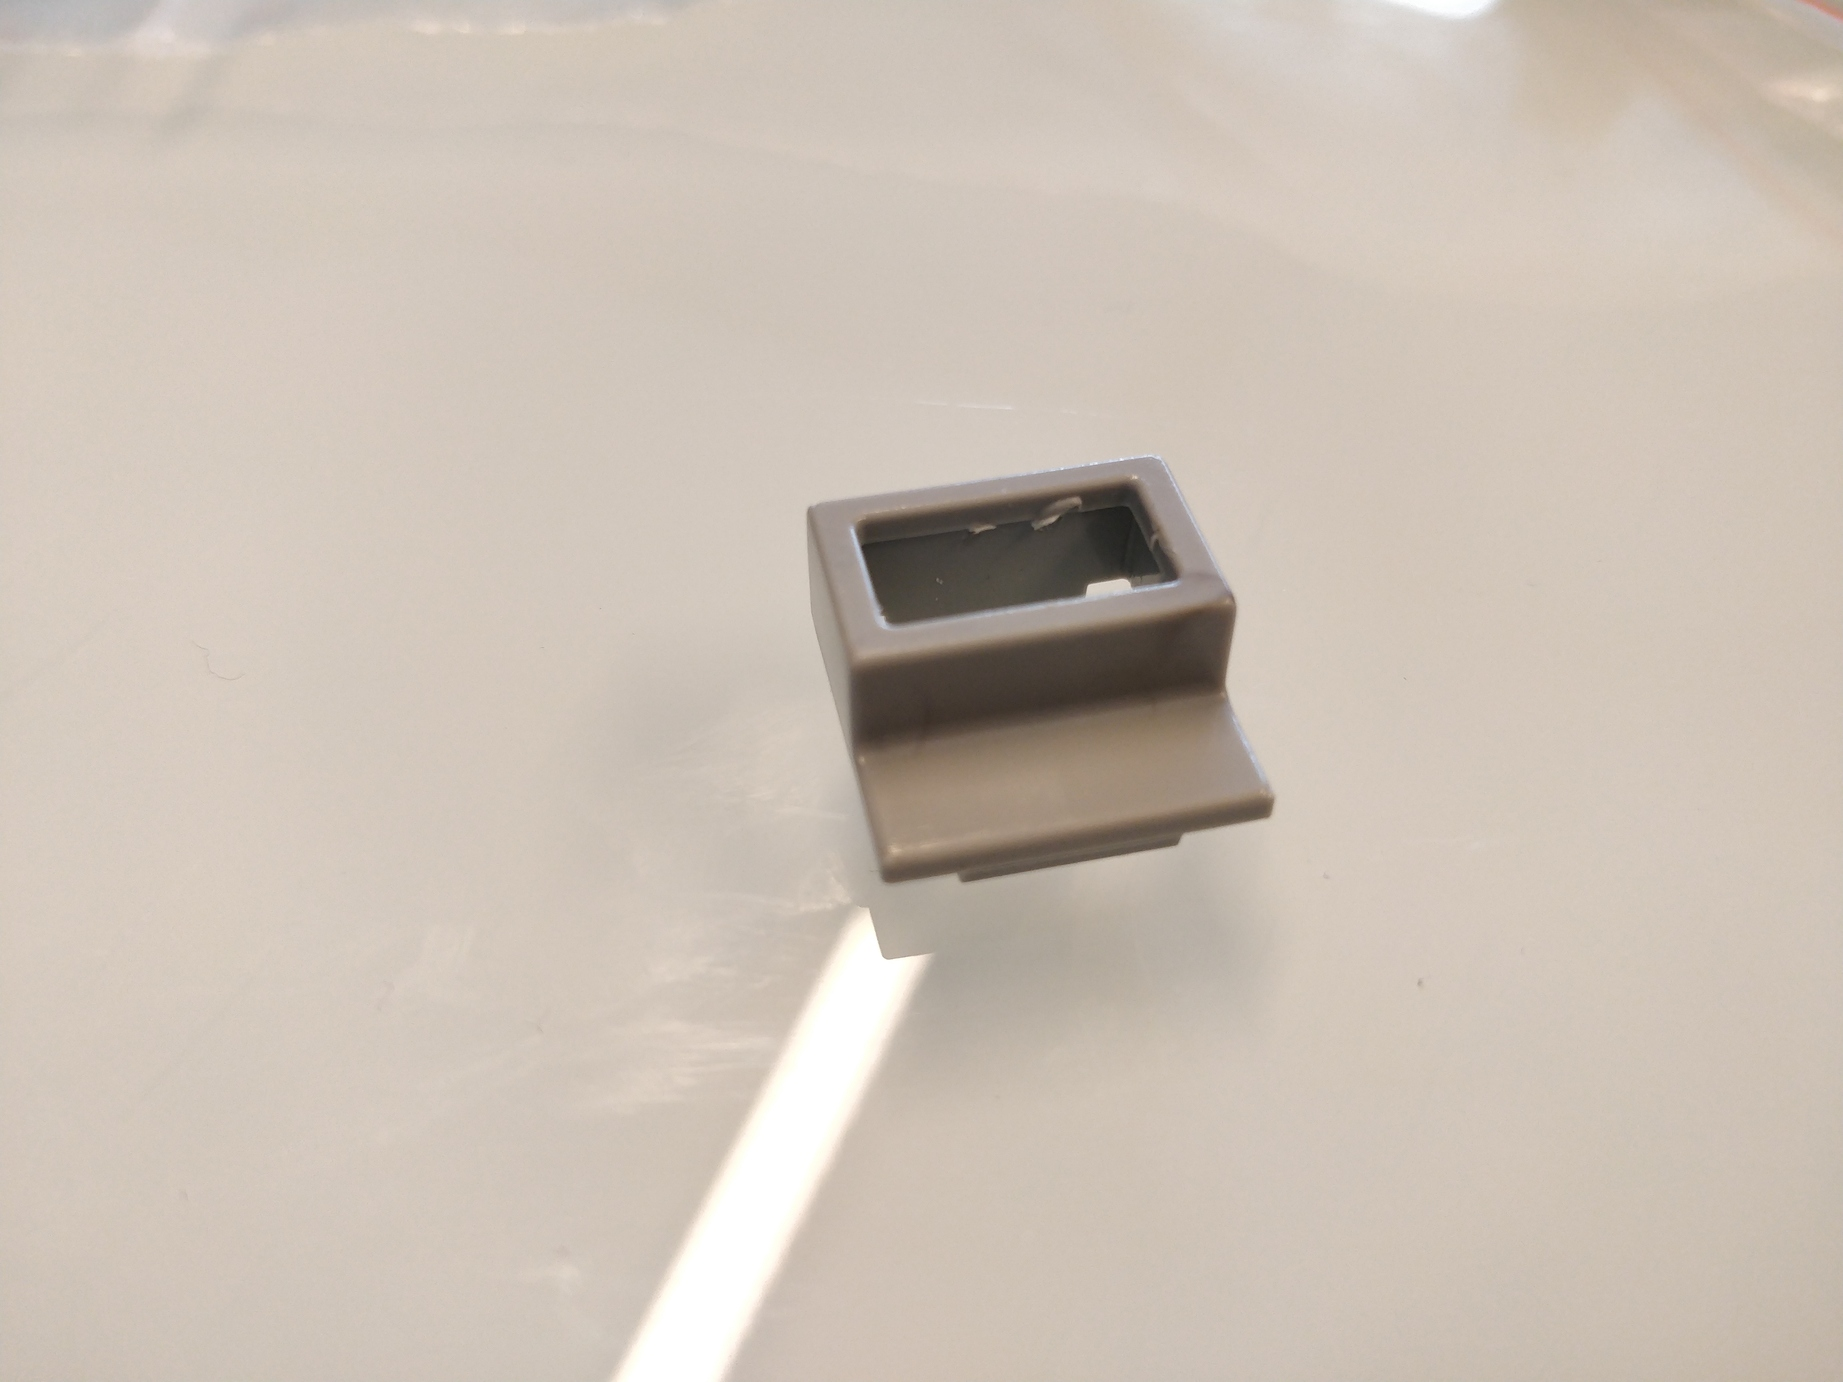
\includegraphics[width=13.5cm]{motor-plastic-top.jpg}

\subsection{Motor adapter case bottom part}

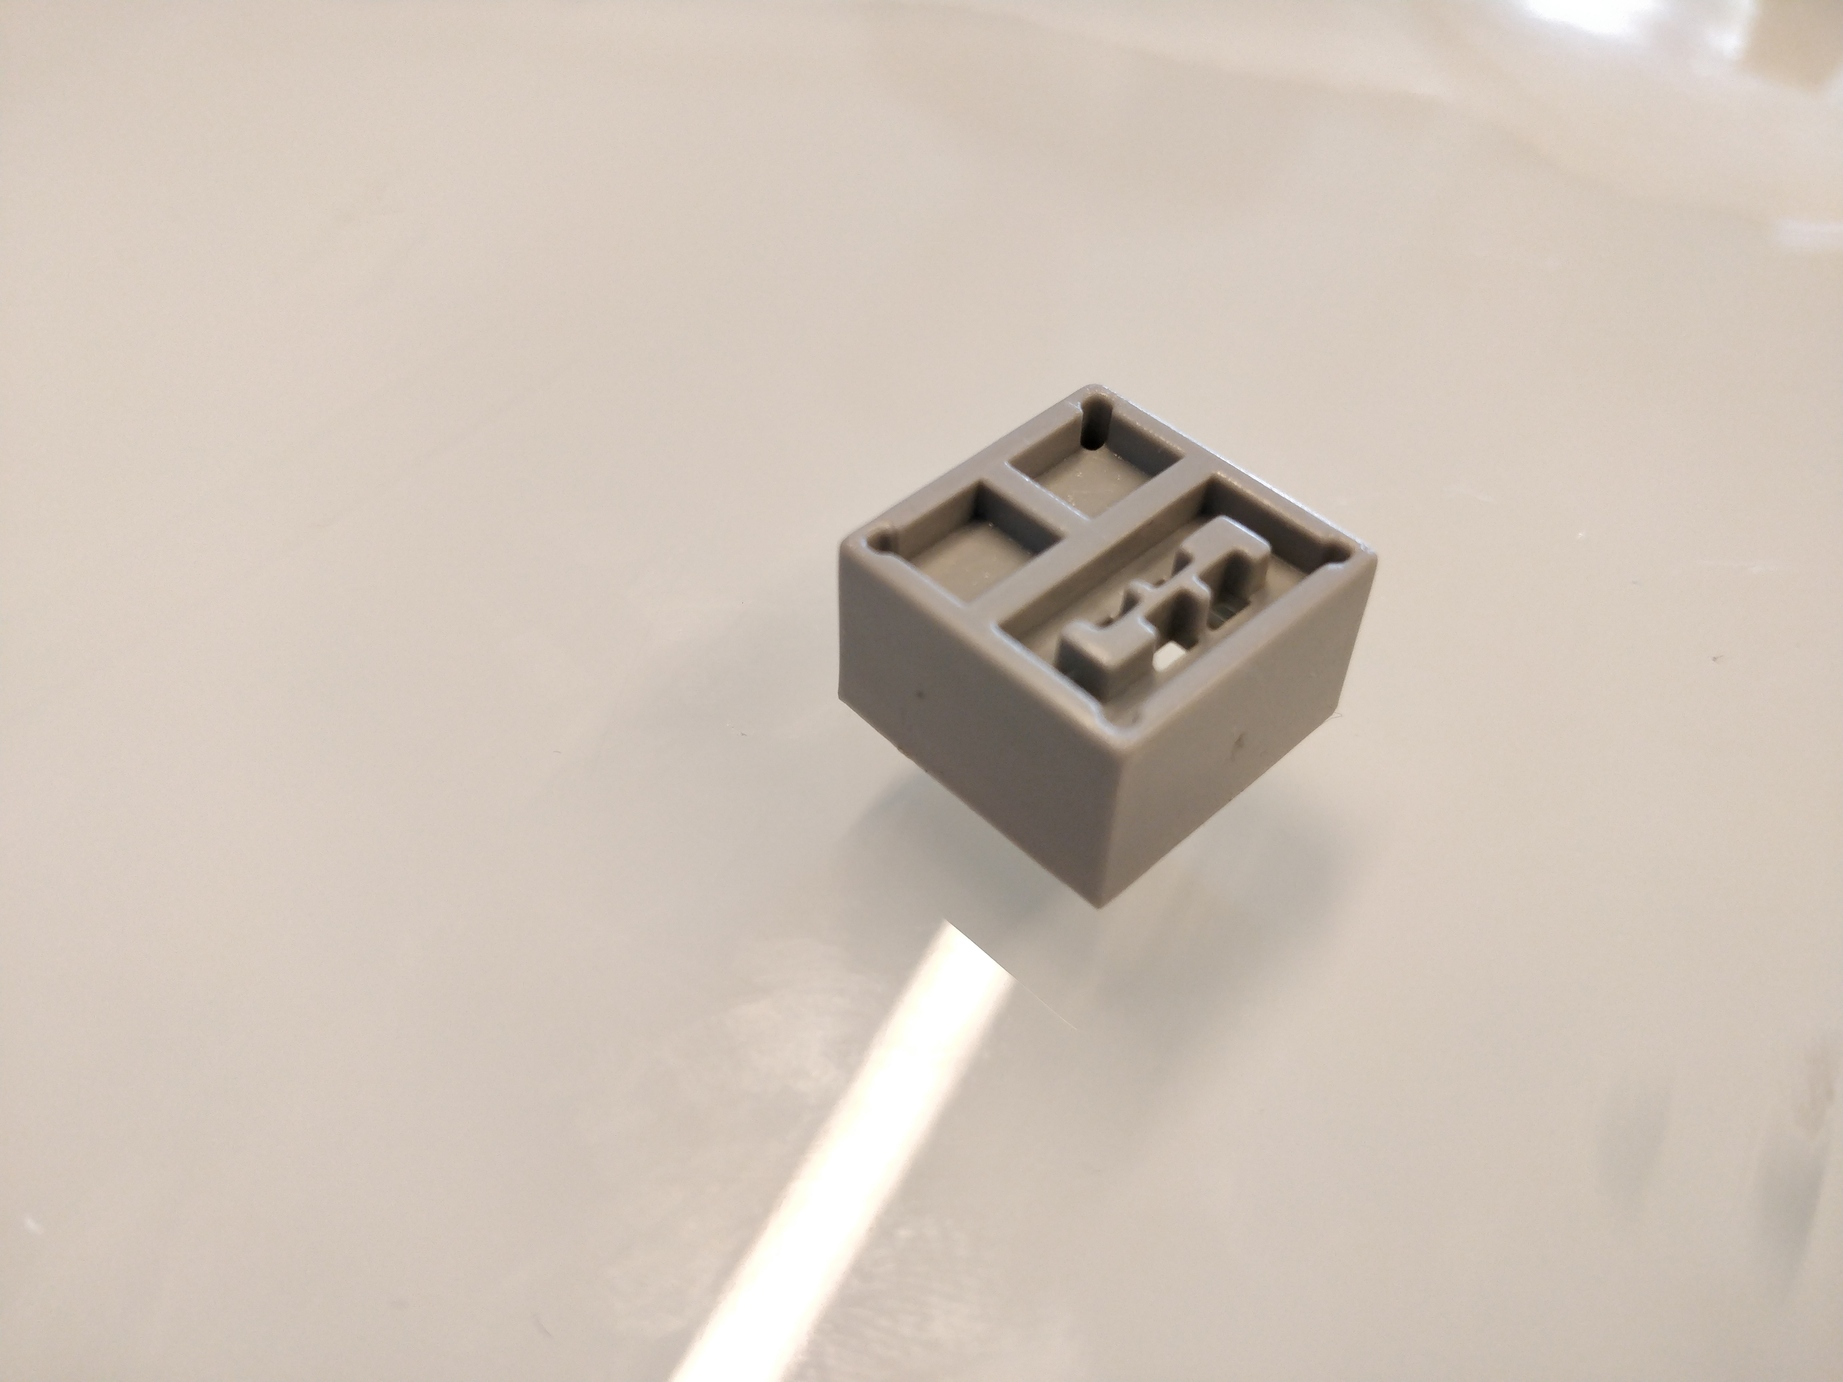
\includegraphics[width=13.5cm]{motor-plastic-bottom.jpg}

\subsection{Sensor adapter case top part}

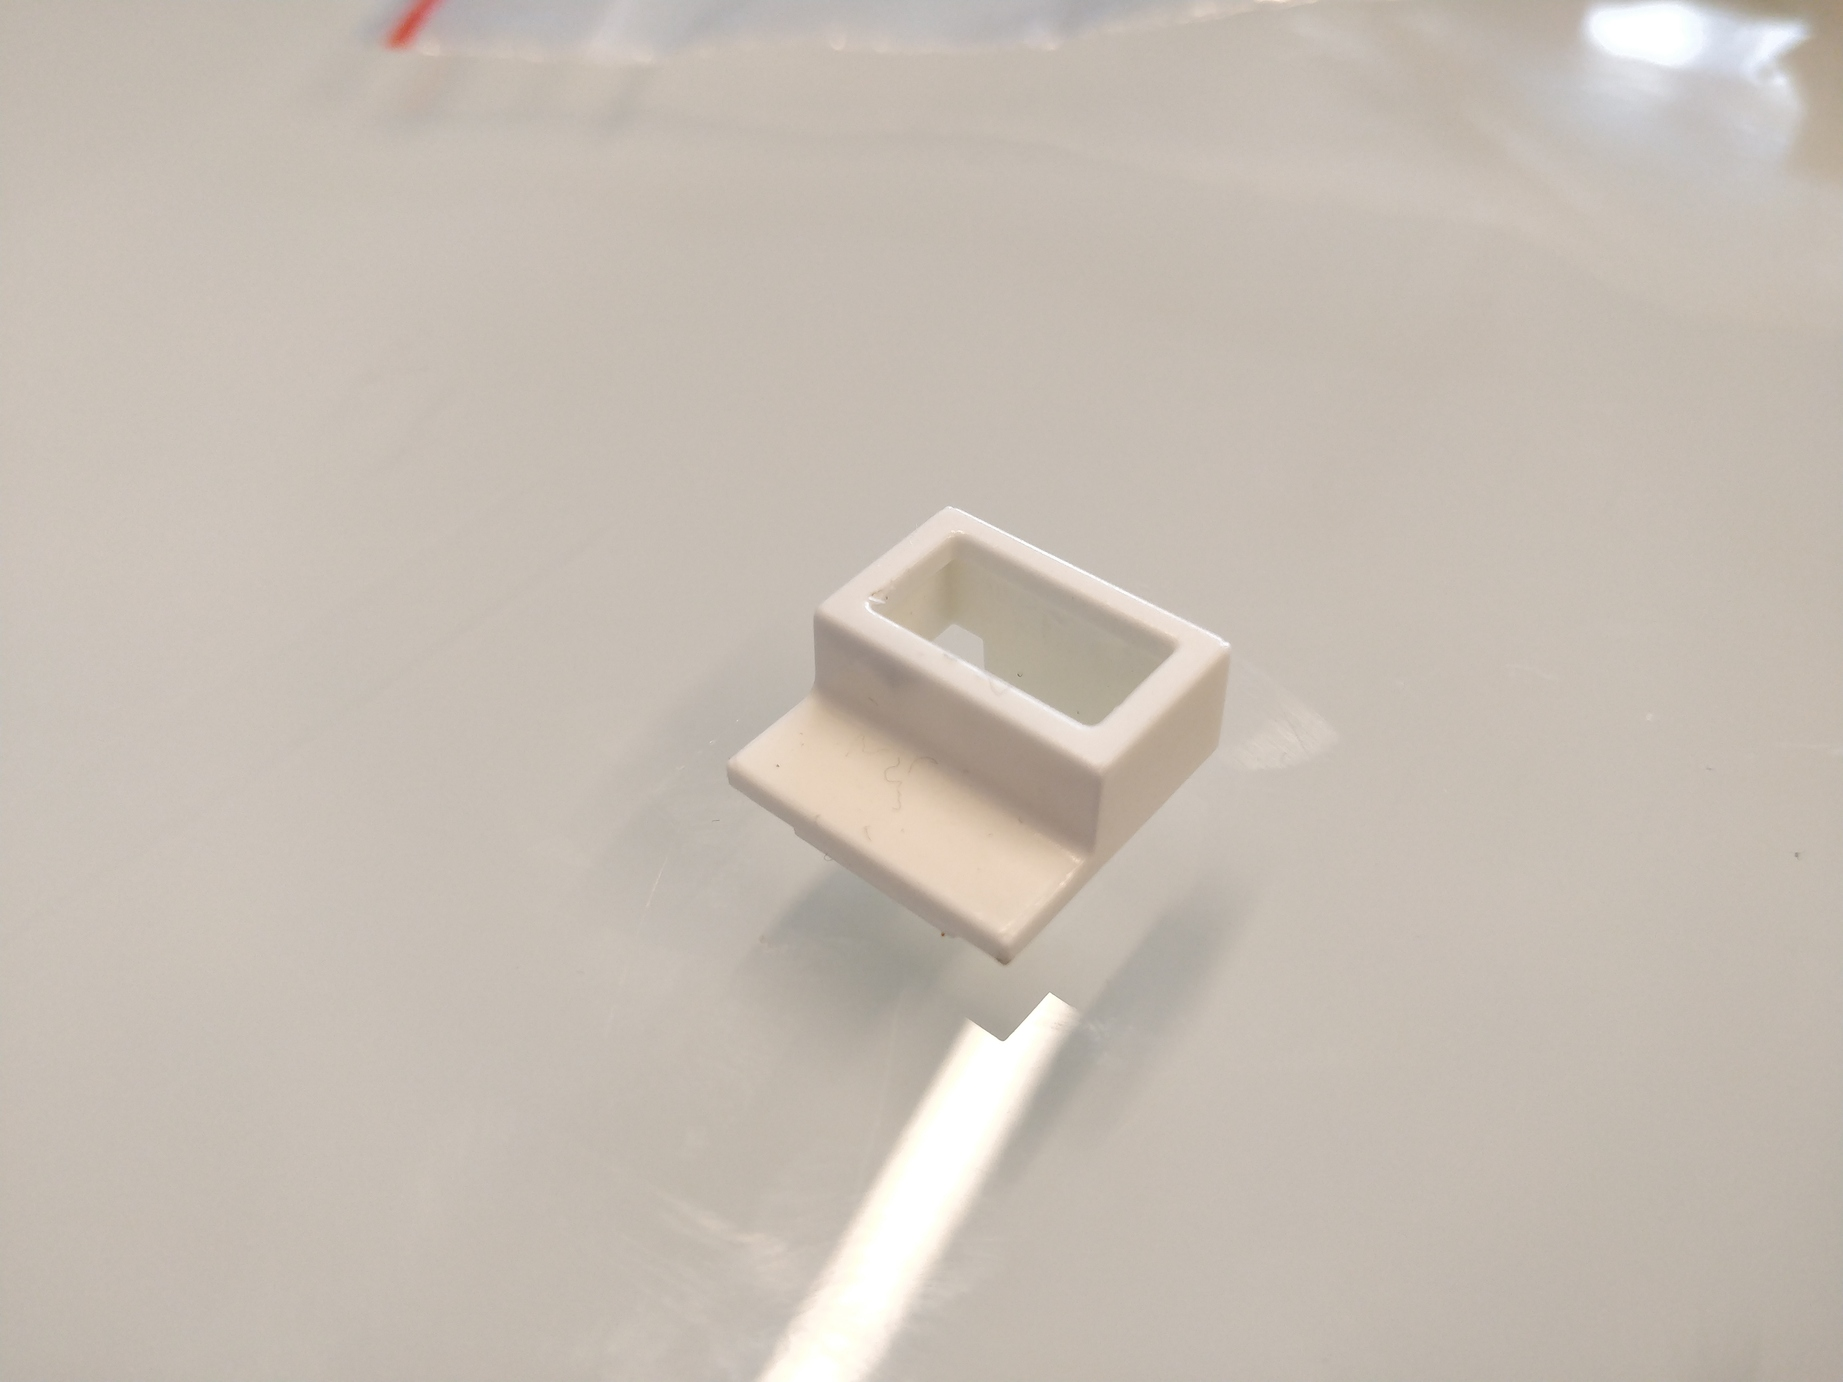
\includegraphics[width=13.5cm]{sensor-plastic-top.jpg}

\subsection{Sensor adapter case bottom part}

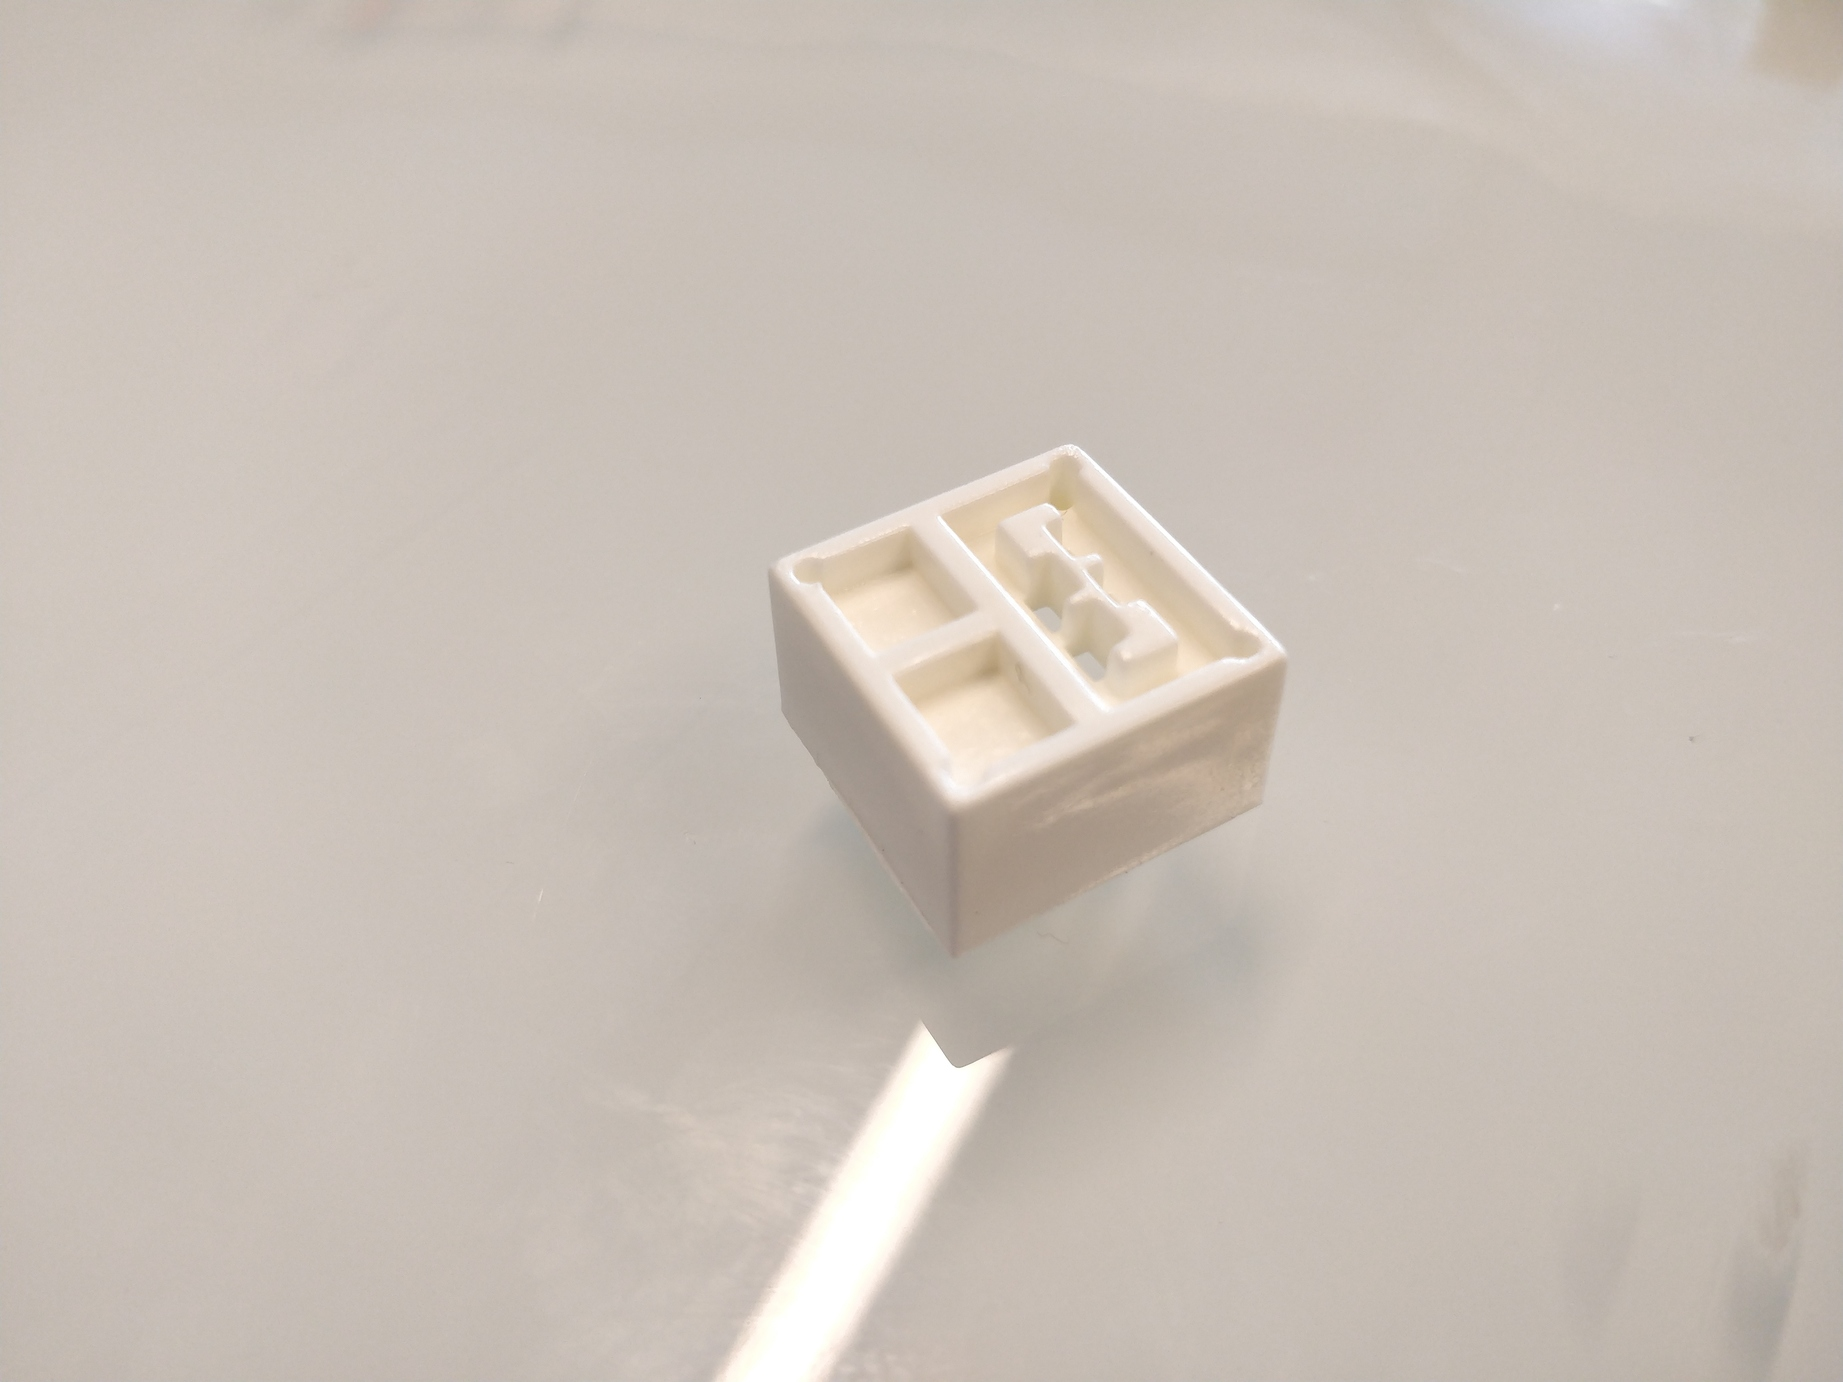
\includegraphics[width=13.5cm]{sensor-plastic-bottom.jpg}

\subsection{EV3 sensor adapter case insert}

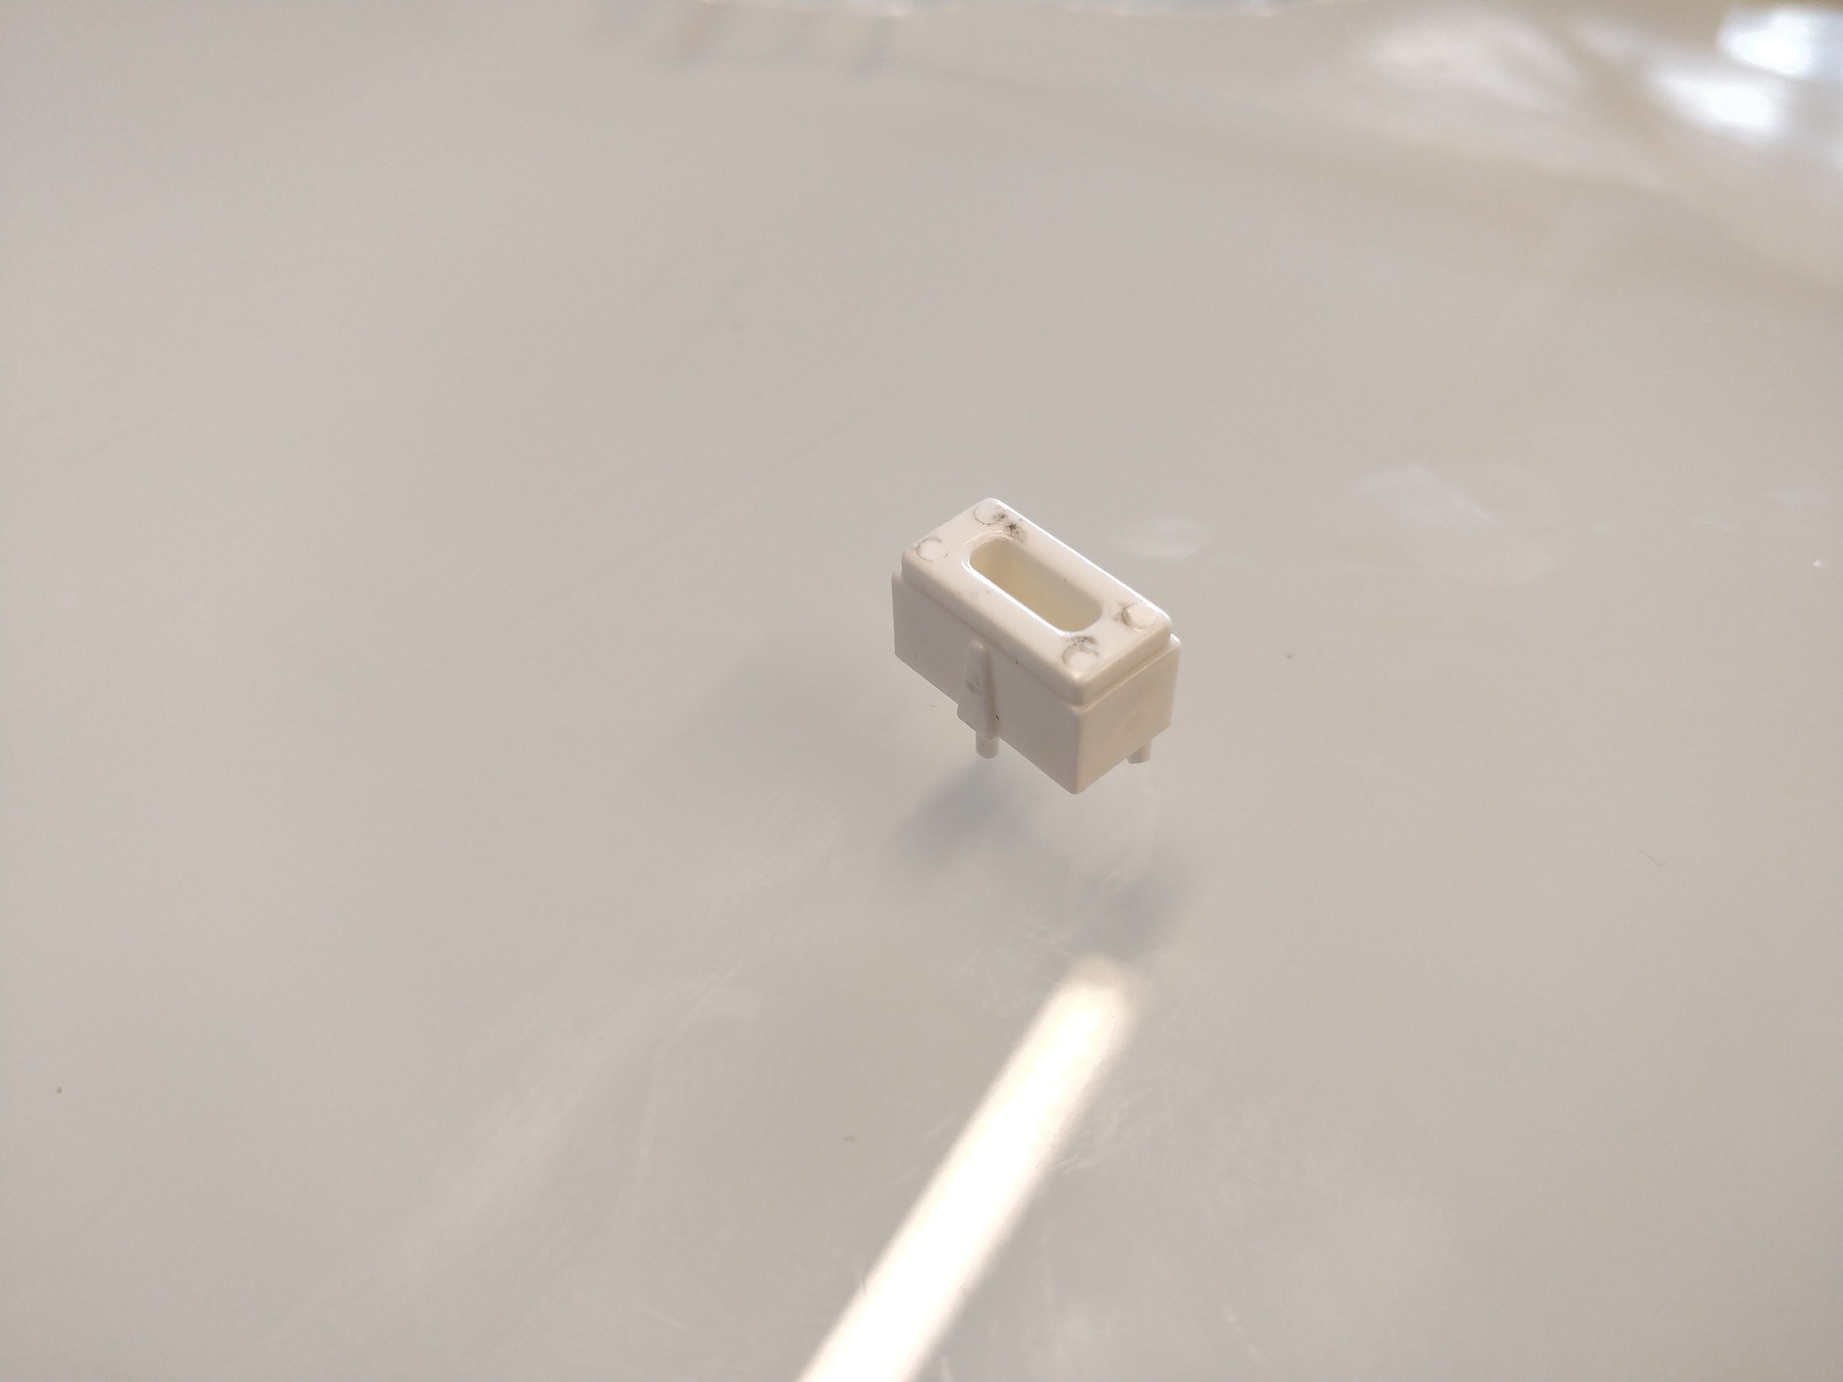
\includegraphics[width=13.5cm]{ev3-sensor-plastic-insert.jpg}

\subsection{Wedo 2 sensor adapter case insert}

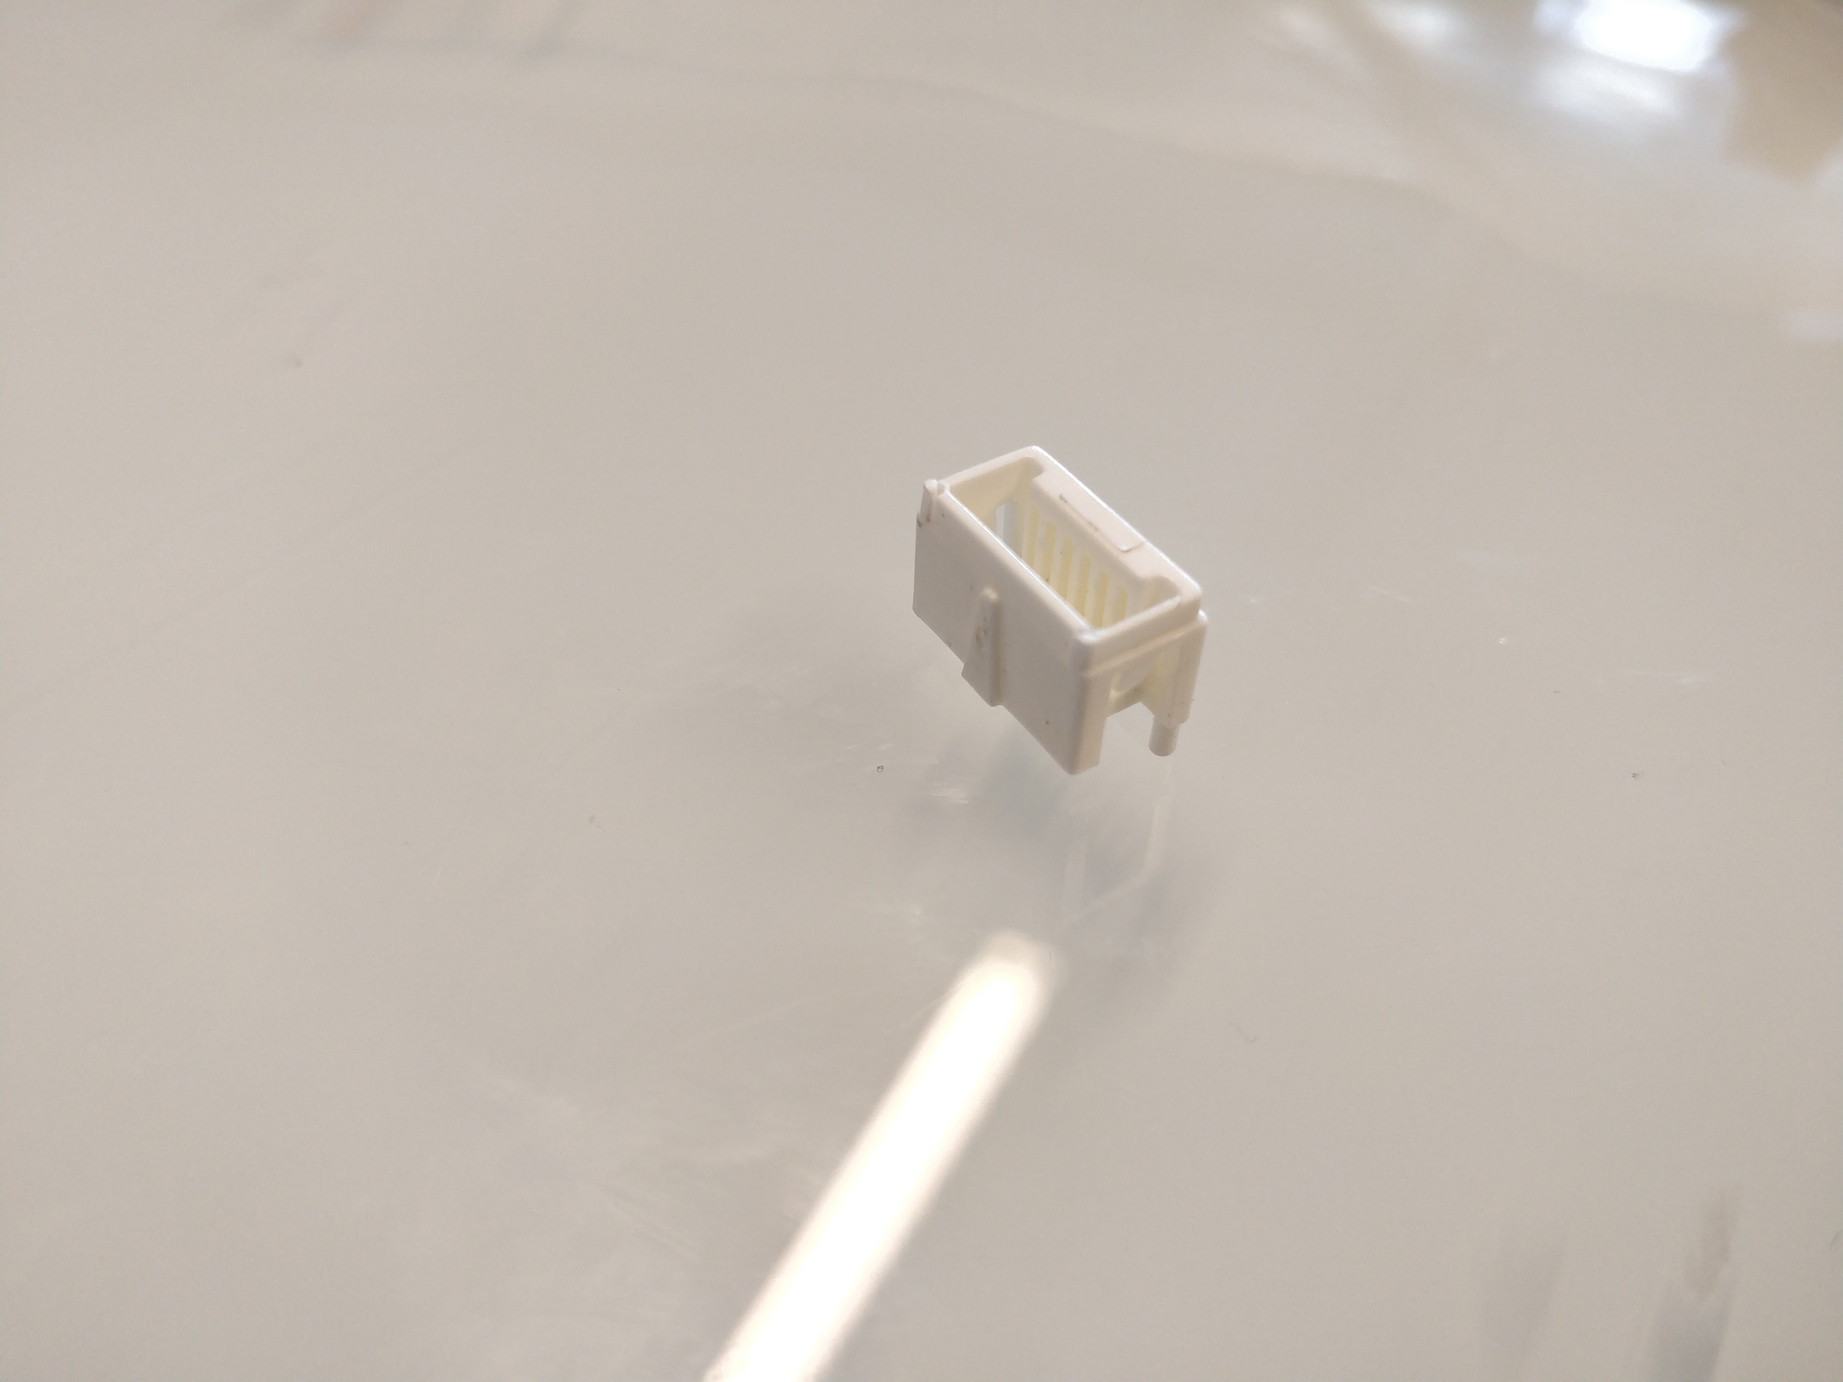
\includegraphics[width=13.5cm]{wedo2-sensor-plastic-insert.jpg}

\subsection{EV3 adapter crimp-on connector}

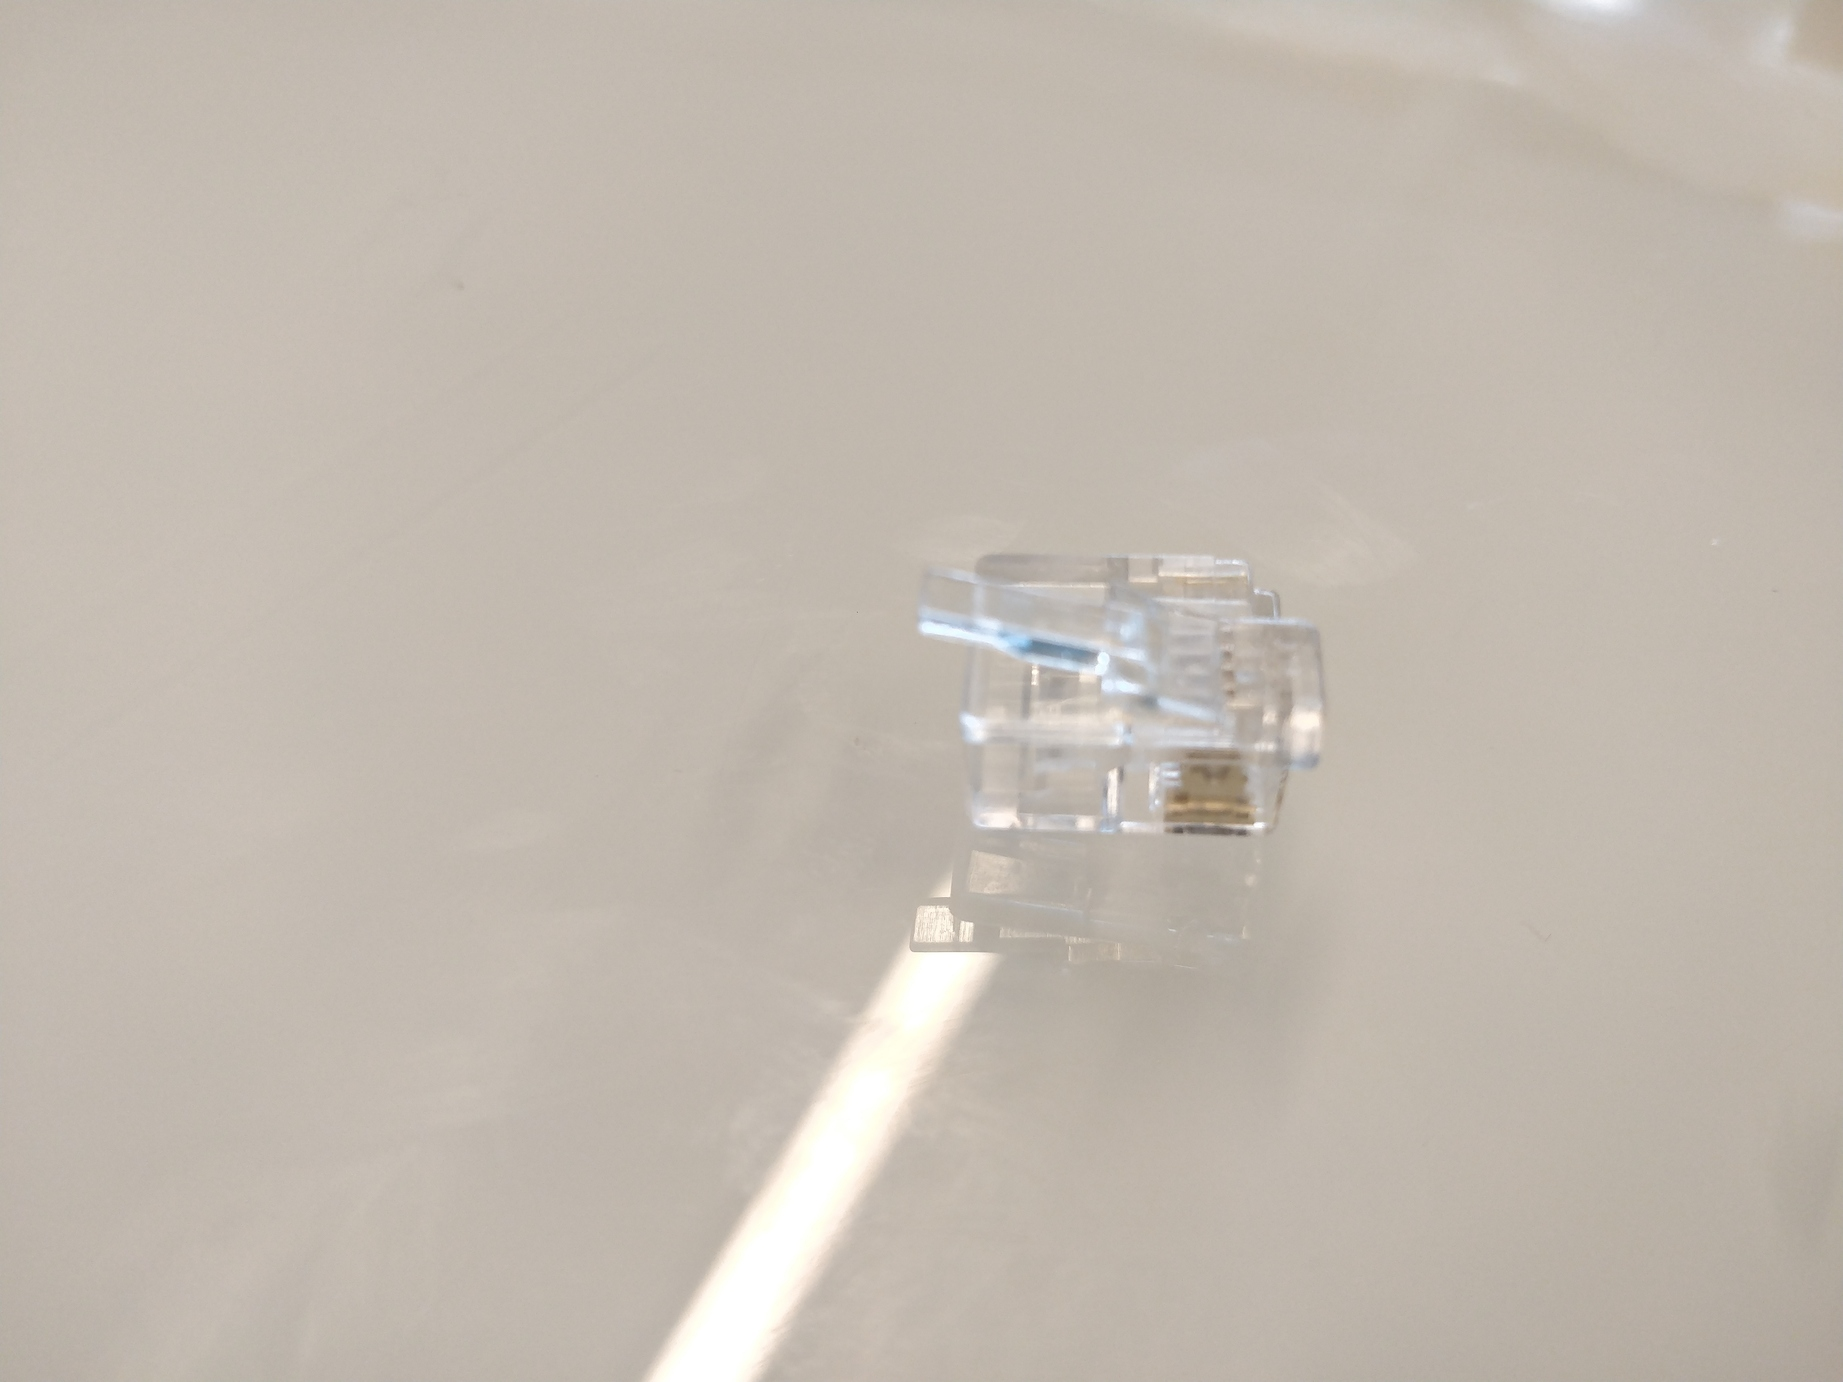
\includegraphics[width=13.5cm]{ev3-connector.jpg}

\subsection{EV3 adapter cable}

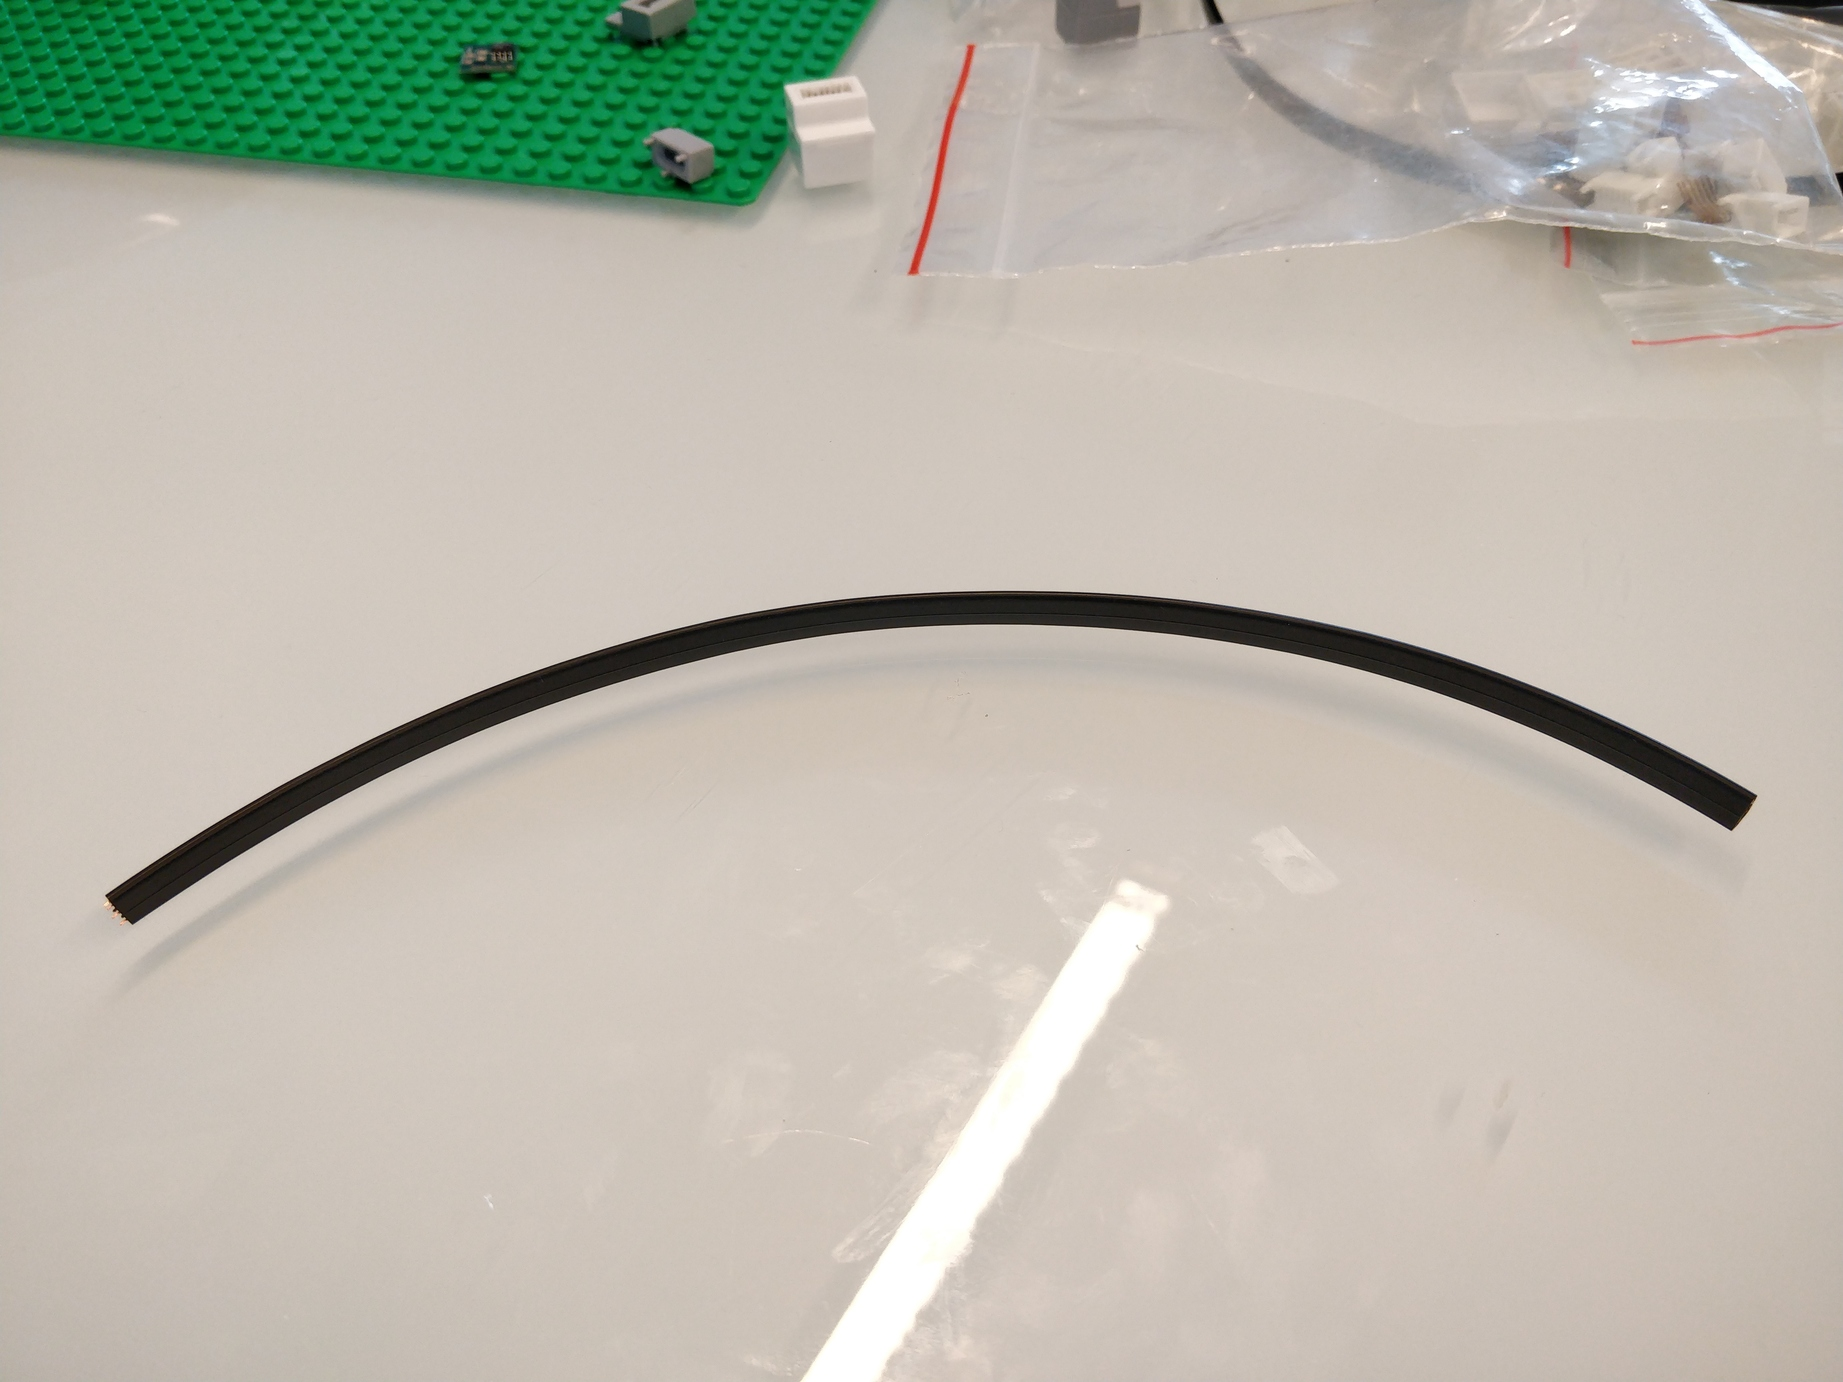
\includegraphics[width=13.5cm]{ev3-cable.jpg}

\subsection{Super glue}

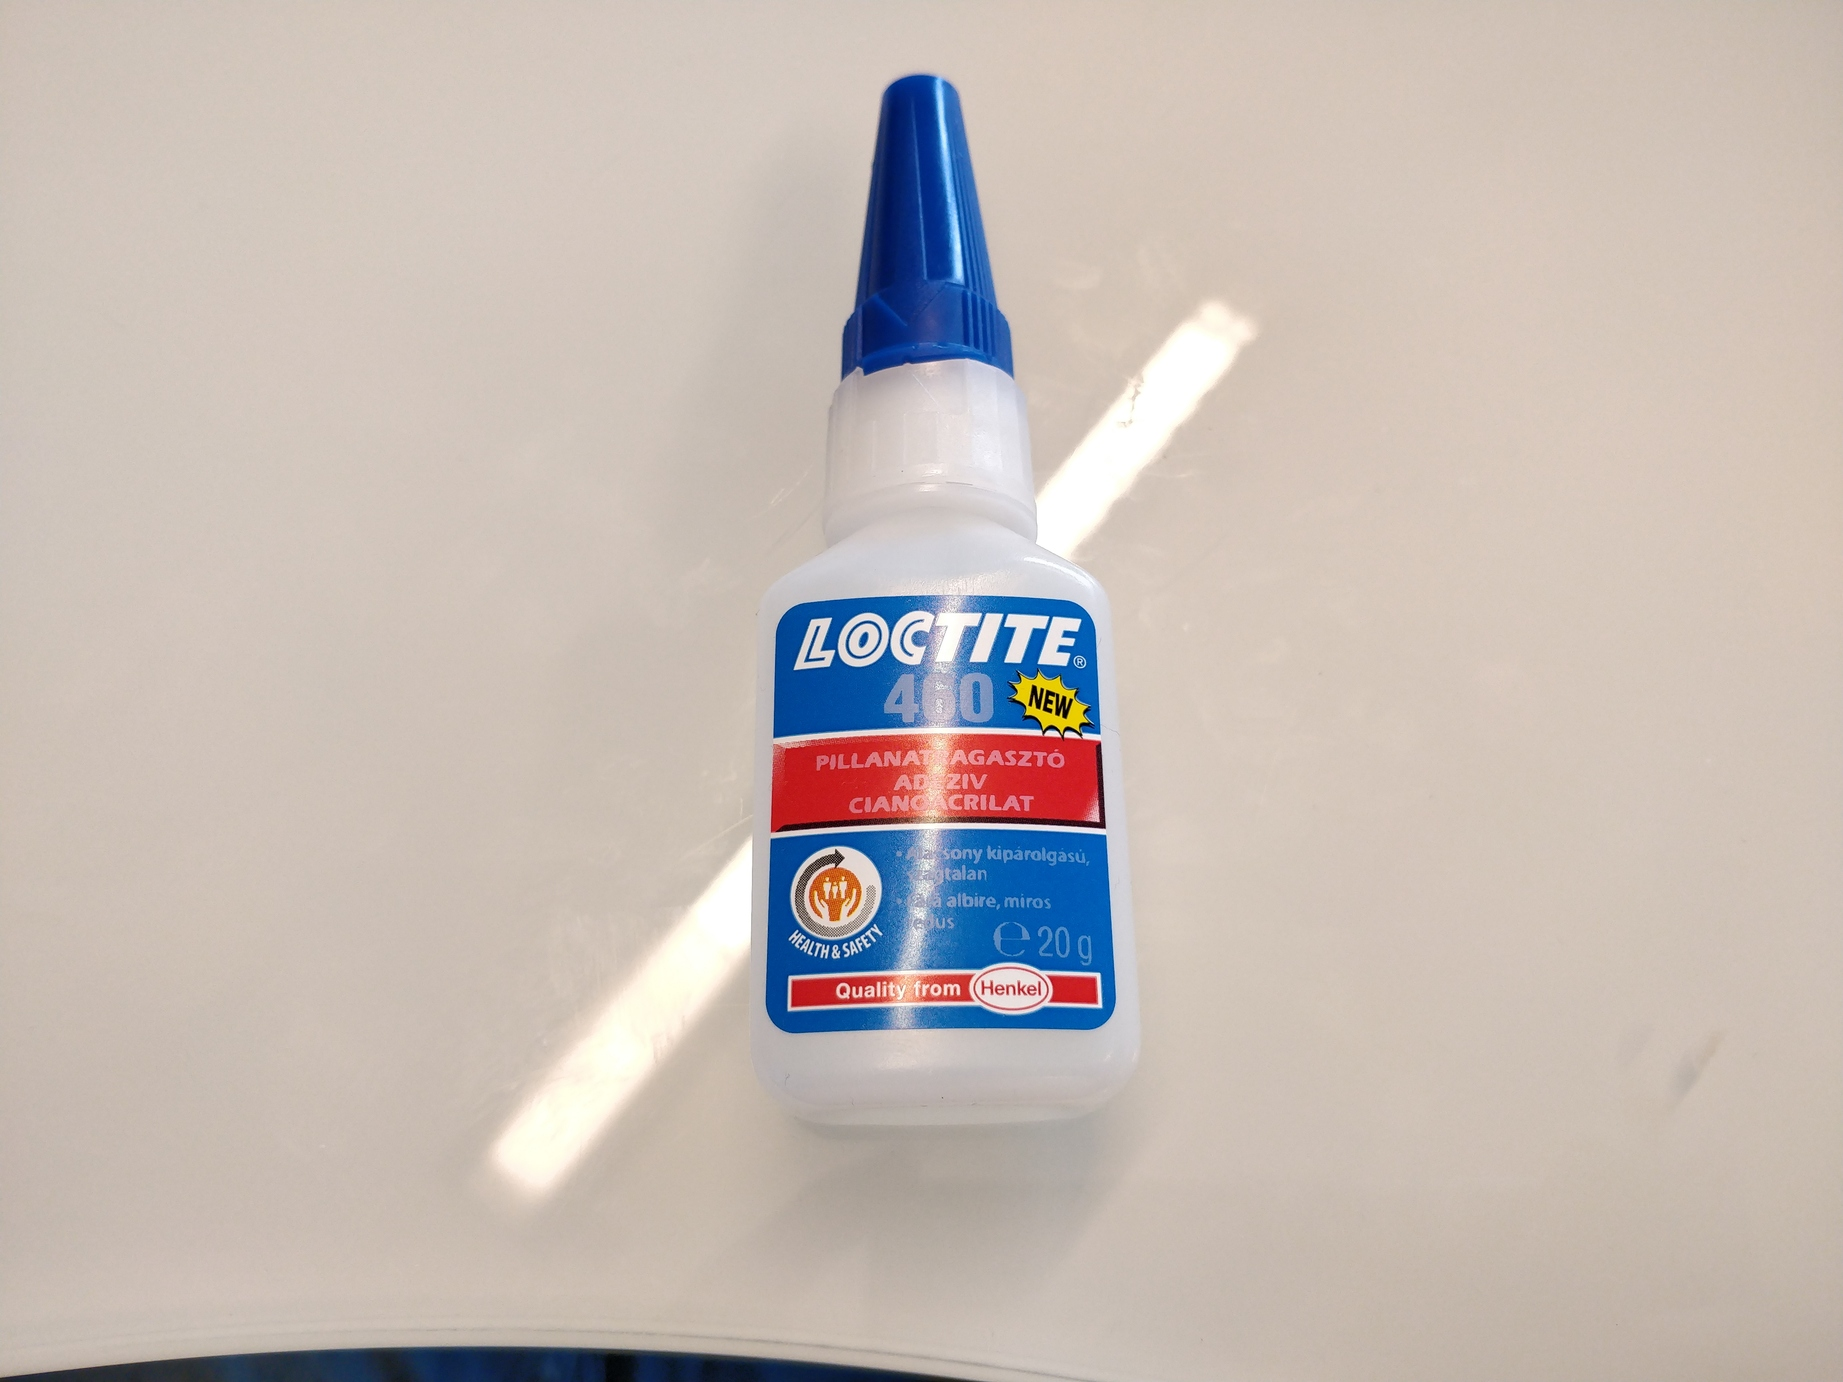
\includegraphics[width=13.5cm]{superglue.jpg}

\subsection{assembled EV3 sensor adapter}

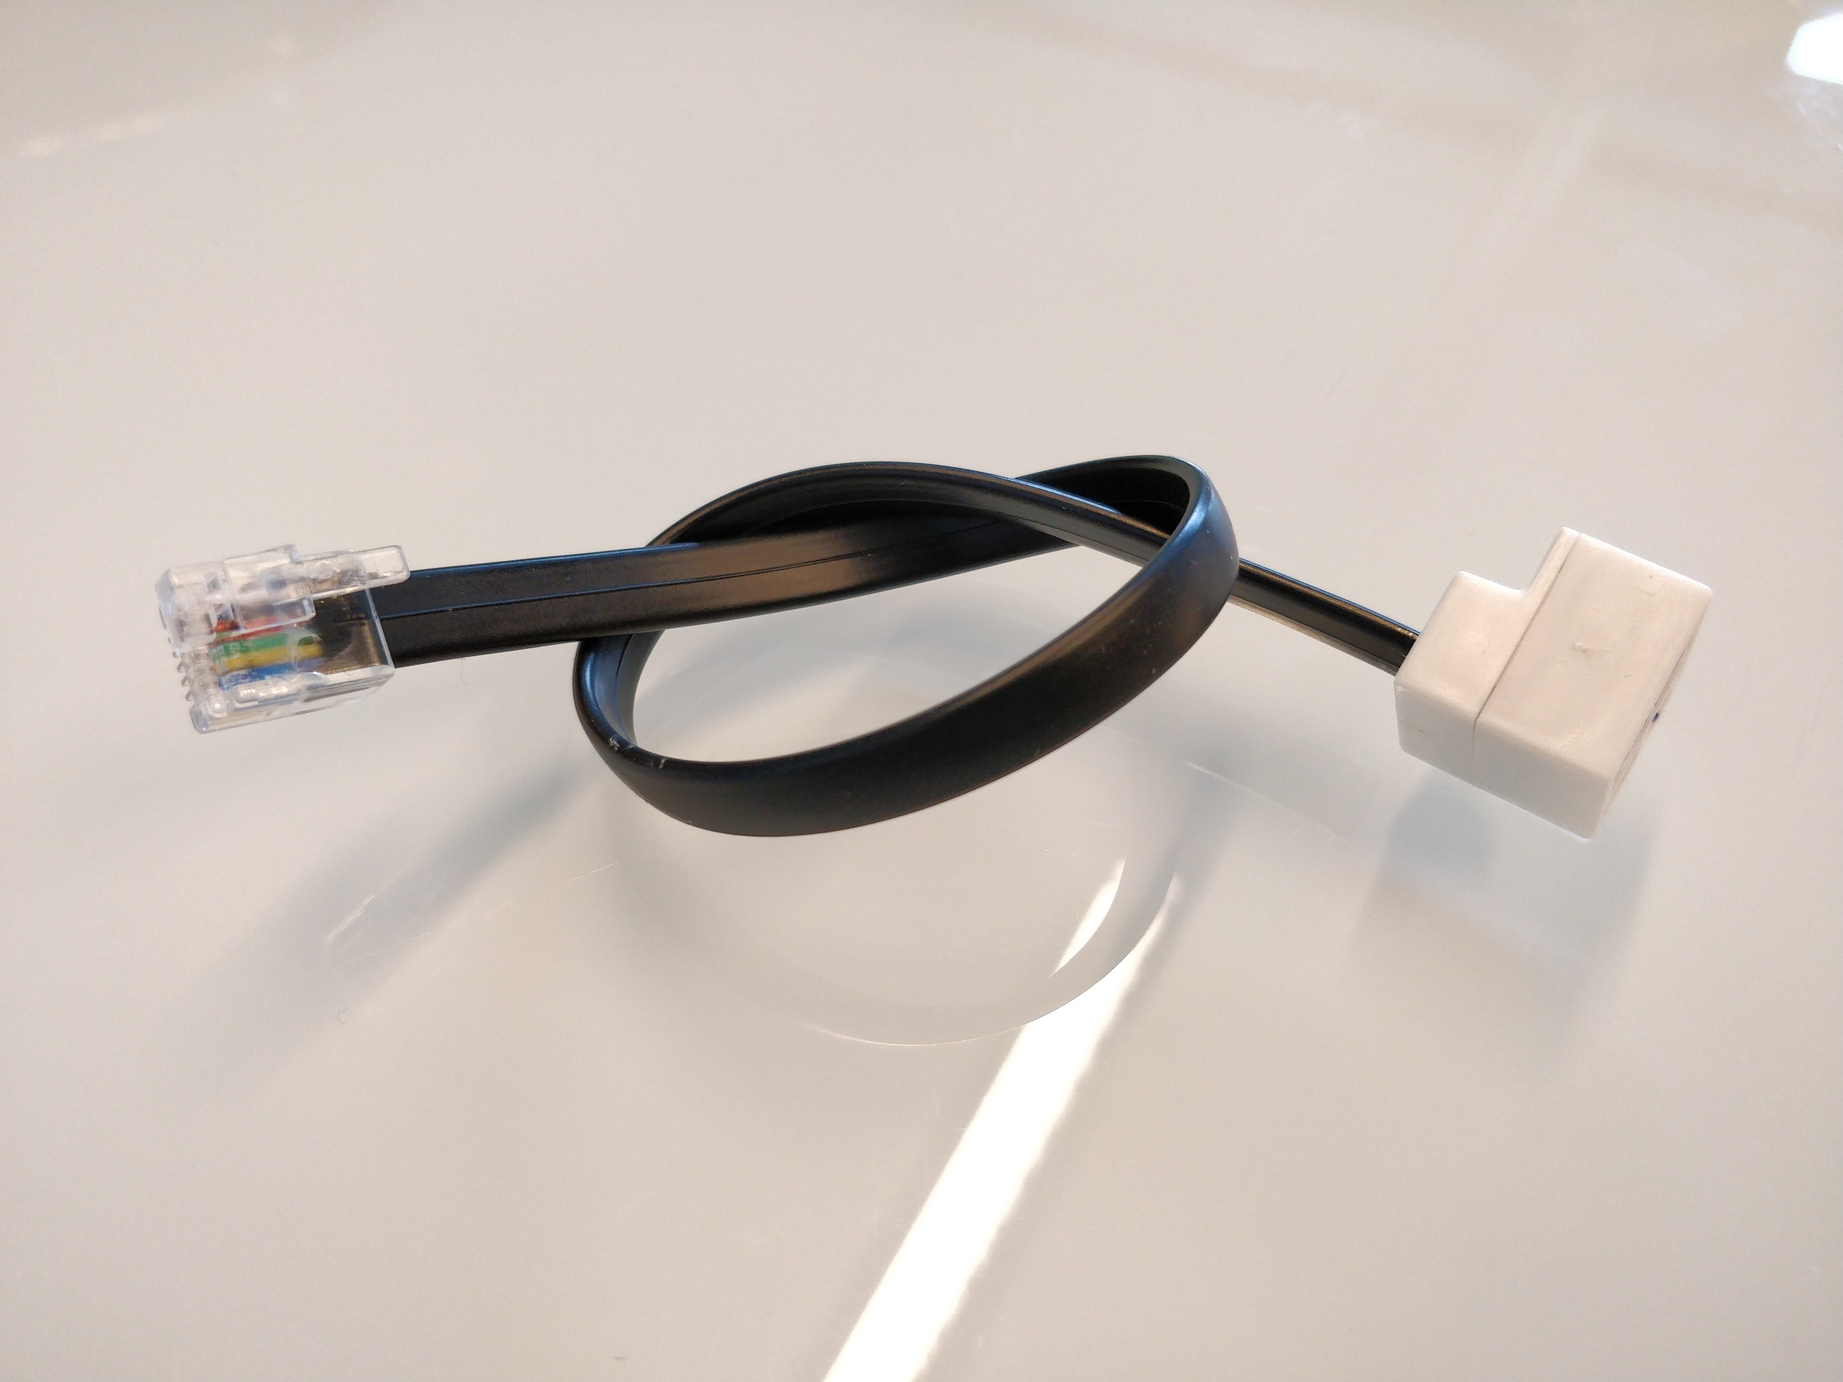
\includegraphics[width=13.5cm]{ev3-sensor-adapter.jpg}

\subsection{Assembled WeDo2 sensor adapter}

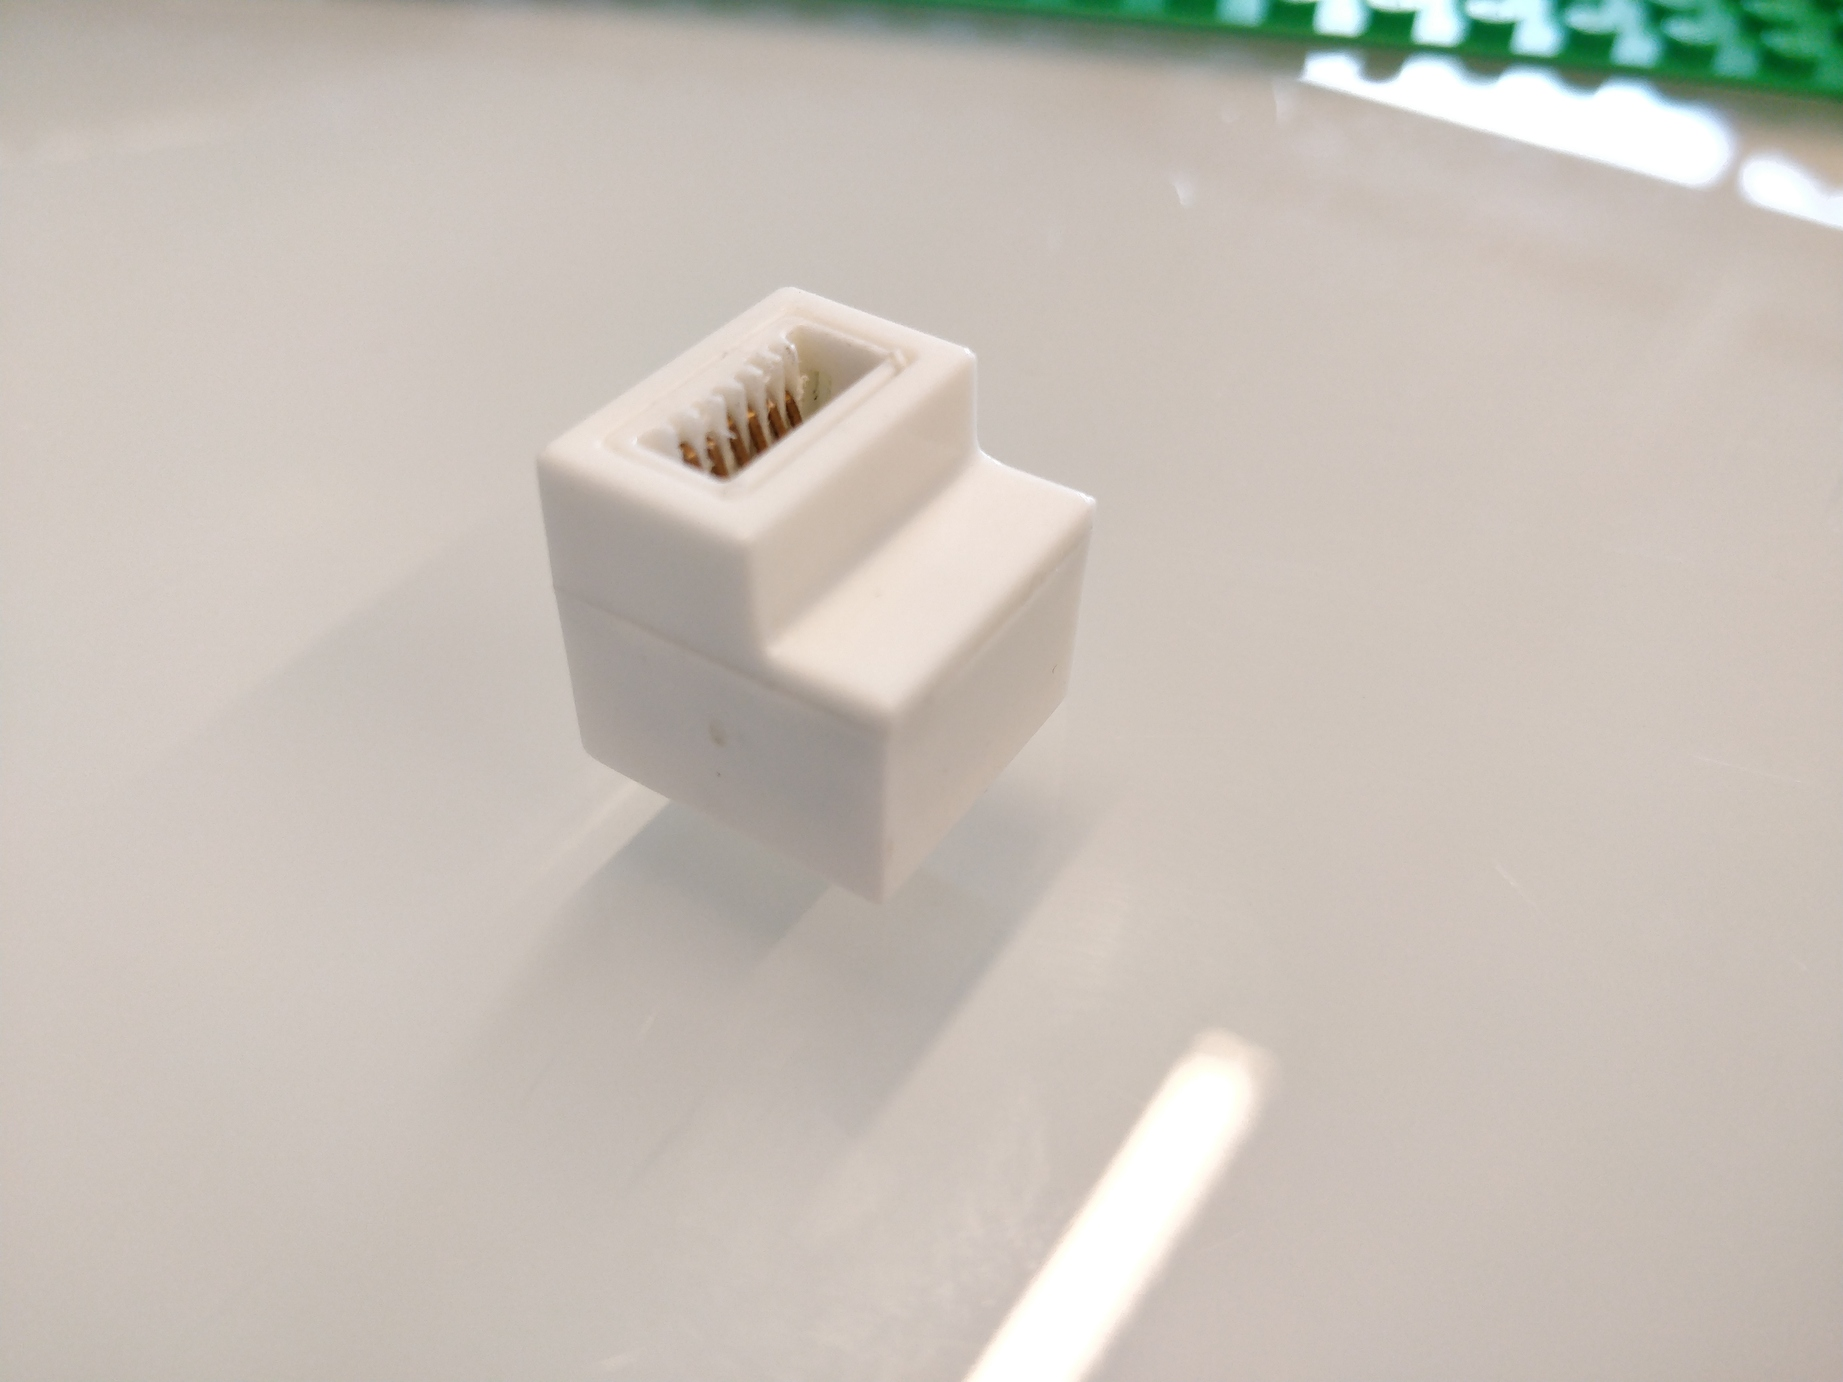
\includegraphics[width=13.5cm]{wedo2-sensor-adapter.jpg}

\subsection{Assembled EV3 motor adapter}

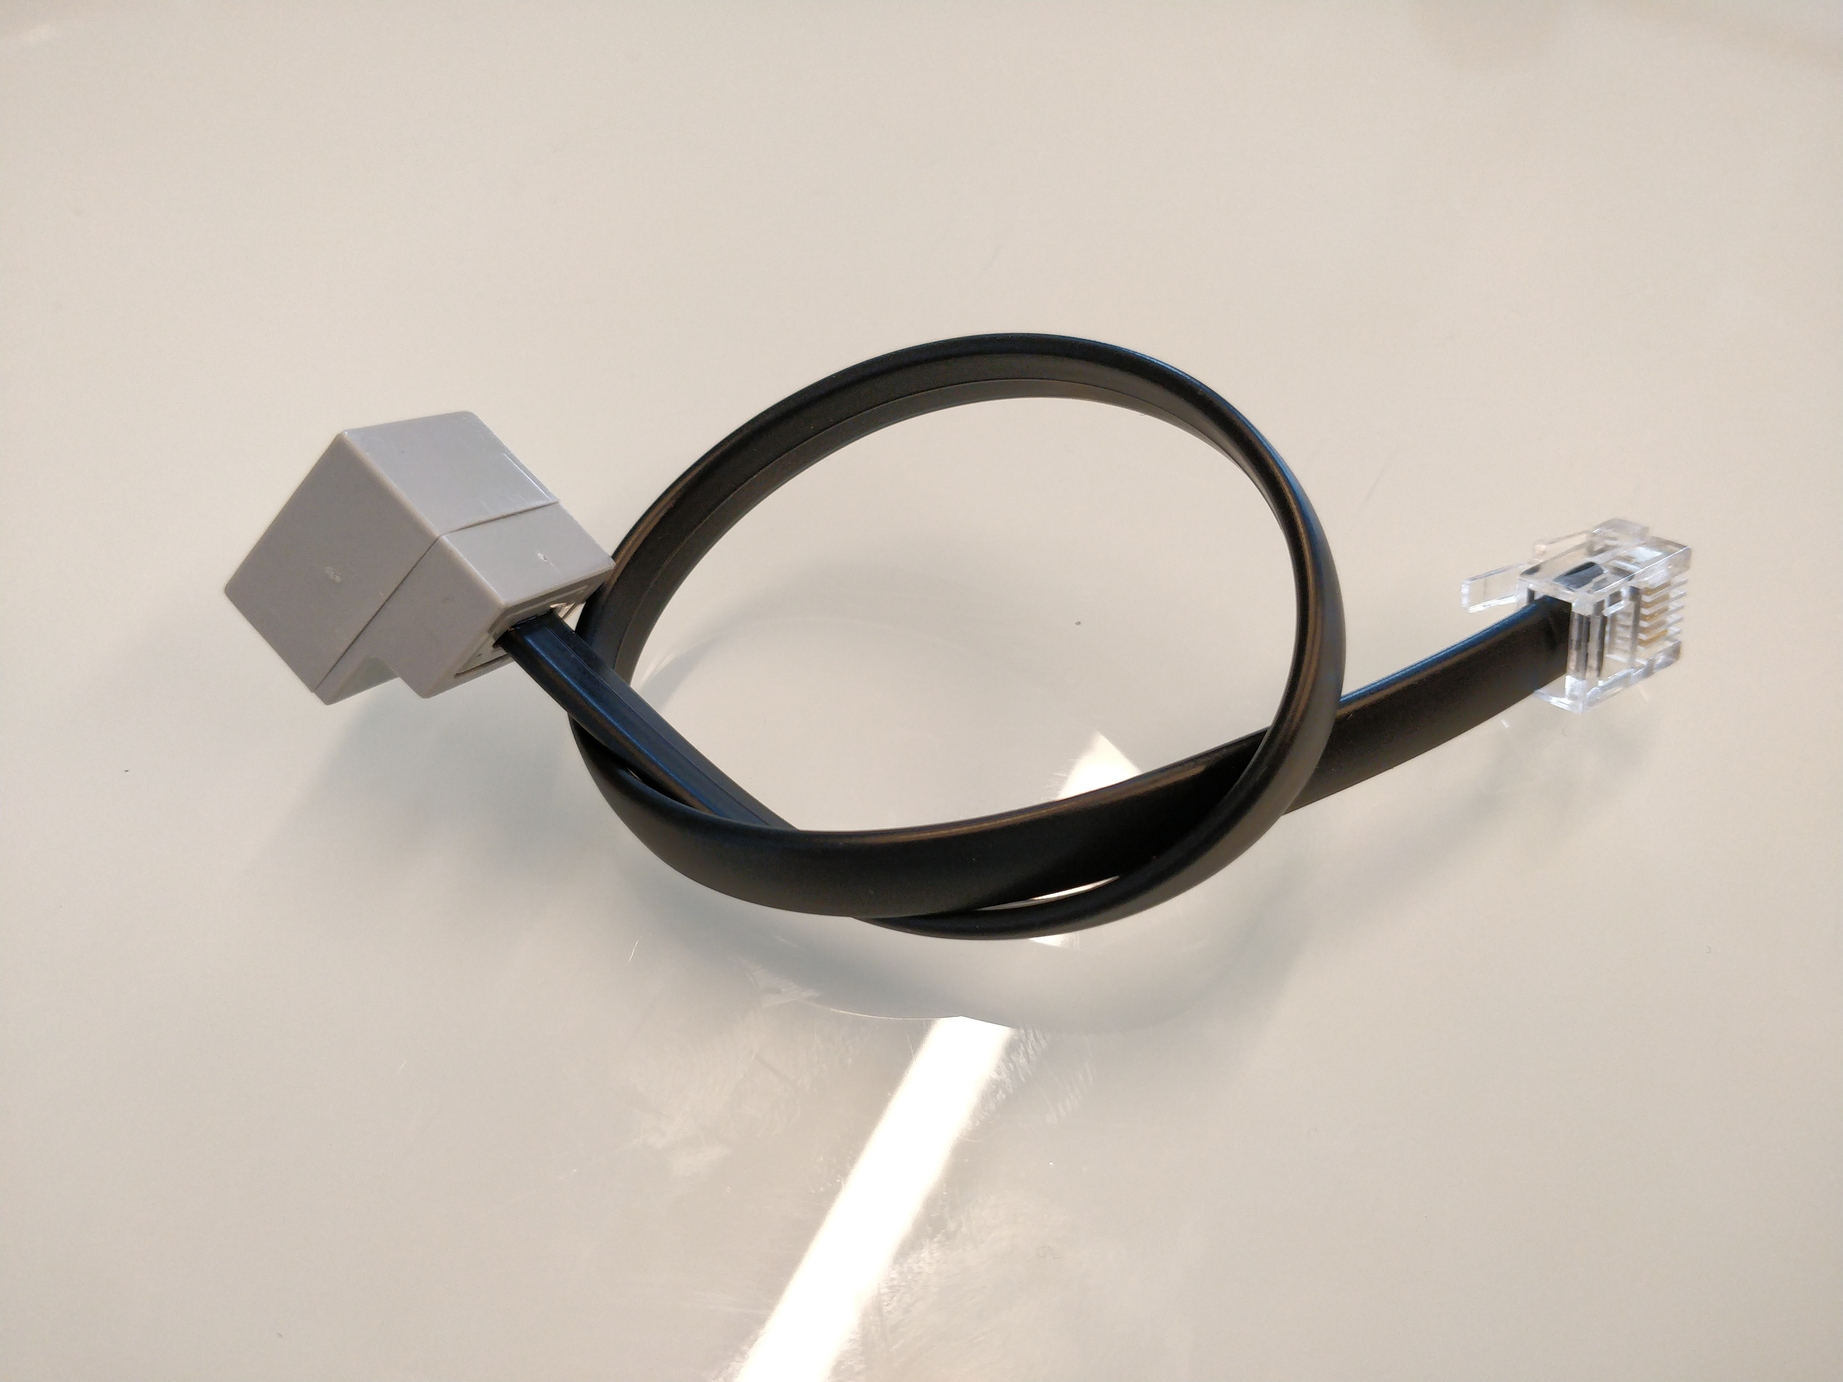
\includegraphics[width=13.5cm]{ev3-motor-adapter.jpg}

\subsection{Assembled WeDo2 motor adapter}

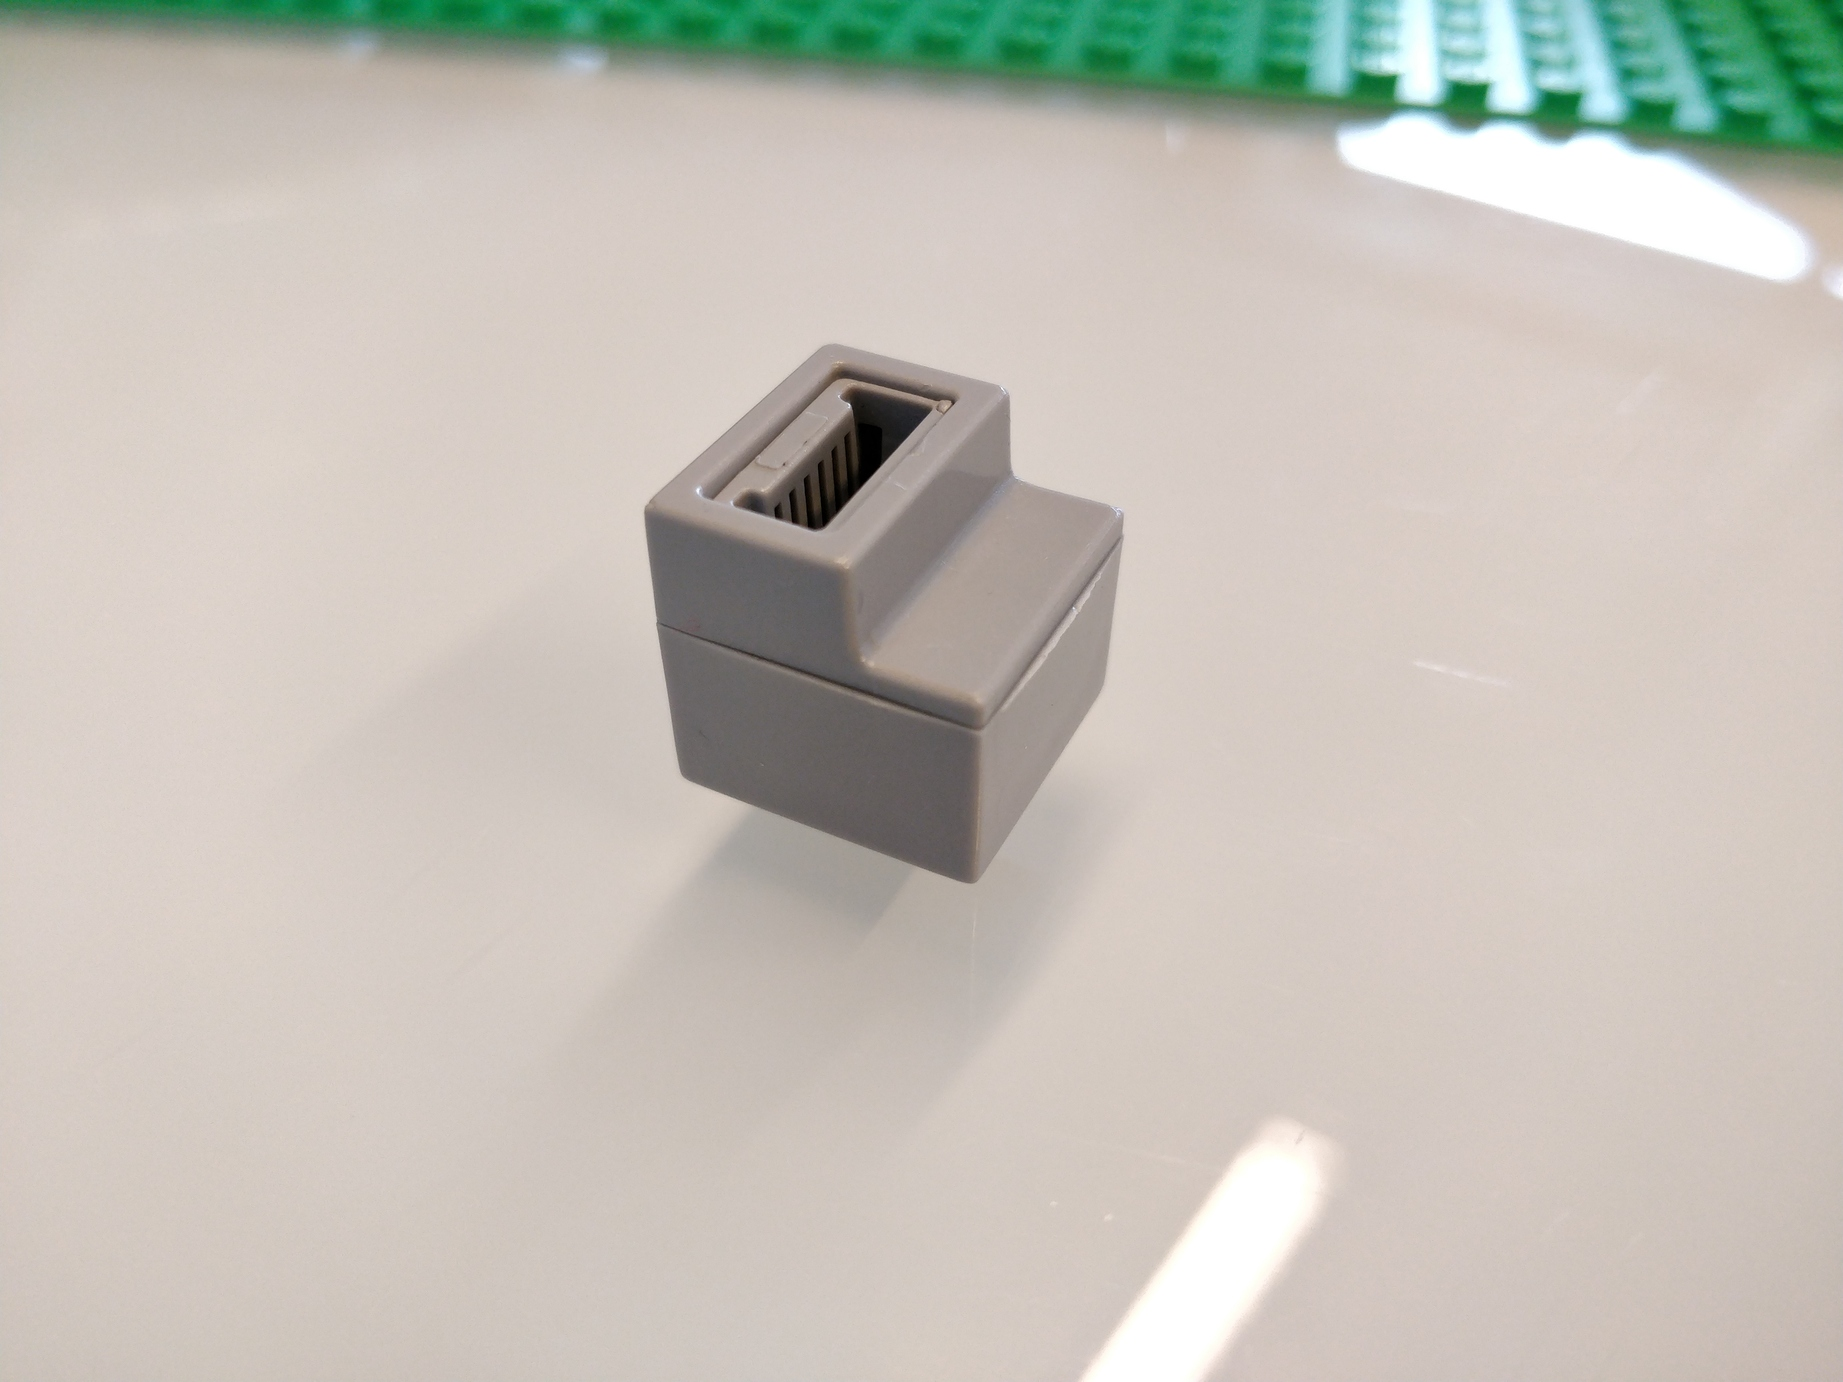
\includegraphics[width=13.5cm]{wedo2-motor-adapter.jpg}

\section{Programming sensor adapters}

During programming, the ATTiny 841 microcontroller receives the firmware and
executes the calibration code for the built-in RC oscillator.

Programming can be done with Microsoft Windows 7 SP1 or more recent operating
system.

Programming is done by executing a .bat file.

The programming hardware consists of an Atmel Ice USB programmer, a power
supply adapter, a power supply, and connecting cables.

The power supply adapter supplies power for the device during programming.
The different sensor adapter require different power supply adapters. EV3
adapters run on 5 volts, while WeDo2 adapters run on 3.3 volts.

\section{Adapter assembly}

\subsection{WeDo 2 adapters}

\begin{enumerate}
    \item Soldering SMD parts and Power Functions pins.

    \item Programming (in the case of sensor adapters).

    \item Soldering WeDo 2 pins.

    \item Fitting the populated board into the plastic case bottom.

    \item Assembly of the plastic case top half: the appropriate insert must be
    inserted into the top part and fixed with a drop of super glue.

    \item Final step: the bottom and top half must be mated by carefully
    inserting the six pins into their respective slots. The two halves must be
    pressed together firmly.
\end{enumerate}

\subsection{EV3 adapters}

\begin{enumerate}
    \item PCB soldering.

    \item Programming (in case of sensor adapters).

    \item Preparation of the cable: both ends of the six-core cable must be
    stripped. All of the conductors must be stripped at one end, only the
    outer jacket have to be stripped at the other end.

    \item Crimping: the connector must be crimped with the appropriate tool.
    Use the end where the individual conductors \emph{are not} stripped.

    \item Assembling the top half: the insert and the plastic case top must
    be mated and secured with a drop of glue.

    \item The top half case must be slided onto the cable.

    \item The stripped conductors must be soldered onto the PCB.

    \item The PCB must be pressed into the plastic case bottom. The plastic
    case top and bottom halves must be pressed together firmly.

    \item The cable jacket and the insert must be glued together.
\end{enumerate}

\end{document}
